%\documentclass[11pt]{report}
%\documentclass[twoside,french,a4,12pt,openright]{MYbook}
%\documentclass[twoside,french,a4,12pt,openright]{book}
\documentclass[twoside,french,a4,12pt,openright]{report}
%\usepackage{utthesis}
%\usepackage[latin1]{inputenc}
\usepackage[french]{babel}
%\usepackage{fancybox}
\usepackage{fancyhdr}
\usepackage{listings}
\usepackage[Lenny]{fncychap}
\usepackage{lmodern}
\usepackage[T1]{fontenc}
\usepackage{charter}
\usepackage{color}
\usepackage{amsmath}
\usepackage{multirow}
\usepackage{tabularx}
\usepackage{colortbl}
%\usepackage{times}
\usepackage{graphicx}
\usepackage{a4wide}
\linespread{1.25}
\begin{document}	

\noindent N$^{\circ}$ D'ORDRE
\pagestyle{empty}
%============= header image ================%
\begin{figure}[htb]
	\centering
	
\includegraphics[width=\columnwidth]{./header}
\end{figure}
%=========================================%

\begin{center}
\setlength\arrayrulewidth{2pt}\arrayrulecolor{blue} 
\setlength\doublerulesep{2pt}\doublerulesepcolor{blue} 
\begin{tabular}{||c||} 
\hline\hline 
\large{TH�SE DE DOCTORAT}\\
\hline\hline 
\end{tabular} 

\setlength\arrayrulewidth{1.5pt}\arrayrulecolor{black} 
\setlength\doublerulesep{1.5pt}\doublerulesepcolor{white} 

%\framebox{\large{TH�SE DE DOCTORAT}}

\vfill

\large{SPECIALITE : PHYSIQUE}\\

\vfill

\textbf{\large{\textit{Ecole Doctorale " Sciences et Technologies de l'Information des T�l�communications et des Syst�mes "}}}\\

\end{center}

\noindent Pr�sent�e par :\\\\
\textbf{Tarik Saidani}

\vfill

\noindent Sujet :
\begin{center}
\textbf{\large{Optimisation Multi-niveau d'Applications de Traitement d'Images sur Machine Parall�le}\\}
\end{center}

\vfill

\noindent Soutenue le ... devant les membres du jury :\\\\

\noindent
M ..\\
M ..\\
M ..\\
M ..\\
M ..\\
M ..\\



%\maketitle
\tableofcontents
\listoffigures
\listoftables
%defining a shade of gray
\definecolor{light-gray}{gray}{0.95}
\definecolor{medium-gray}{gray}{0.80}

\pagestyle{fancy}
\fancyhead[RO,LE]{}

\chapter{Introduction}
�
Les logiciels ont �t� con�us historiquement pour une ex�cution en s�rie. Les programmes devaient s'ex�cuter sur une seule machine contenant une seule unit� de traitement centrale (\emph{CPU}) et le probl�me est d�compos� en une suite d'instructions qui sont ex�cut�es les unes apr�s les autres. Ainsi, une seule instruction peut �tre ex�cut�e � la fois. Le calcul parall�le est par opposition � la pr�c�dente approche, l'utilisation simultan�e de plusieurs ressources de calcul pour r�soudre un probl�me. Un logiciel peut ainsi s'ex�cuter sur plusieurs \emph{CPU}. Le probl�me est d�compos� en plusieurs parties qui peuvent �tre r�solues de mani�re concurrente. Ces parties sont � leur tour d�compos�es en plusieurs instructions et chaque paquet d'instructions s'ex�cute de mani�re ind�pendante l'un de l'autre. Les ressources de calculs incluent une seules machine avec plusieurs processeurs, un nombre arbitraire de machines connect�es via un r�seau ou alors une combinaison des deux. Une bonne partie des probl�mes de calcul intensif poss�dent certaines caract�ristiques qui en font de bon candidats � la parall�lisation. Parmi ces caract�ristiques: le possibilit�s de les d�composer en plusieurs sous-probl�mes qui peuvent �tre r�solus simultan�ment et la possibilit�s d'�tre r�solus en moins de temps avec plusieurs ressources qu'avec une seule. Le calcul parall�le �tait auparavant, r�serv� exclusivement � la mod�lisation de probl�mes et de ph�nom�nes scientifiques provenant de la r�alit� tels que l'environnement, la physique nucl�aire, les biotechnologies, la g�ologie et les math�matiques. A ce jour, le calcul parall�le s'est ouvert � d'autre domaines gr�ce notamment � l'�volution fulgurante de la technologie des semi-conducteurs qui a rendu les plate-formes haute performance plus accessibles. On peut citer des applications comme les bases de donn�es, l'exploration p�troli�re, les moteurs de recherche, la mod�lisation financi�re, les technologies de diffusion multim�dia et les applications graphiques et de r�alit� virtuelle.
\subsection{Concepts G�n�raux}
\subsubsection{Architecture de \emph{von Neumann}}
\begin{figure}[!htb]
	\centering
	\includegraphics[width=0.6\columnwidth]{Chapter1/figures/vonneumann}
	\caption{Architecture de \emph{von Neumann}}
	\label{figvonneumann}
\end{figure}
Ce mod�le fut invent� par le math�maticien hongrois \emph{John von Neumann} qui a pos� les premi�res bases de la conception d'un ordinateur dans son papier de 1945 \cite{vonneumann}. A partir de ce moment tous les ordinateurs ont �t� con�us sur ces bases. L'architecture \emph{von Neumann} \ref{figvonneumann} est constitu�e de 4 composants principaux: une m�moire, une unit� de contr�le, une unit� arithm�tique et logique(\emph{ALU}) des Entr�es/Sorties (\emph{I/O}). La m�moire � acc�s al�atoire (\emph{RAM}) en lecture/�criture est utilis�e pour stocker les instructions ainsi que les donn�es. L'unit� de contr�le va chercher les instructions ou les donn�es de la m�moire, d�code les instructions et coordonne s�quentiellement les op�rations afin d'accomplir la t�che programm�e. L'ALU effectue les op�rations arithm�tiques de base. les I/O font l'interface avec l'utilisateur humain.
\subsubsection{Classification de Flynn des Machines Parall�les}
Il existe plusieurs mani�res de classer les machines parall�les. Toutefois, il existe une classification qui est largement utilis�e depuis 1966 et qui est celle de Flynn \cite{flynn} (\emph{Flynn's Taxonomy}). Cette classification distingue les architectures parall�les selon deux param�tres ind�pendants qui sont les instructions et les donn�es : chacun de ces deux param�tres peut avoir deux �tats possibles \emph{Single} ou \emph{Multiple}. Ainsi le tableau \ref{flynn} illustre la classification de Flynn.
\begin{table}
\centering
\begin{tabular}{|c||c|}
\hline
\textbf{SISD} &  \textbf{SIMD} \\
\hline
Single Instruction Single Data& Single Instruction Multiple Data\\
\hline
\hline
\textbf{MISD} &  \textbf{MIMD} \\
\hline
Multiple Instruction Single Data& Multiple Instruction Multiple Data\\
\hline
\end{tabular}
\caption{Classification de Flynn des machines parall�les}
\label{flynn}
\end{table}

\paragraph{Single Instruction, Single Data (SISD)}
Une machine s�rie qui ne peut ex�cuter qu'un seul flux d'instruction en un cycle d'horloge \emph{CPU}. De plus, un seul flux de donn�es est utilis� comme entr�e en un cycle d'horloge. L'ex�cution du programme y est d�terministe et il constitue le type de machines � la fois le plus ancien est le plus r�pandu de nos jours.
\paragraph{Single Instruction, Multiple Data (SIMD)}
C'est un type de machines parall�les dont les processeurs ex�cutent la m�me instruction en un cycle d'horloge donn�. Cependant, chaque unit� de traitement peut op�rer sur un �l�ment de donn�es diff�rent. Ce type de machines est bien taill� pour des probl�mes r�guliers tels que le traitement d'images et le rendu graphique. L'ex�cution des programme y est synchrone et d�terministe. Deux variantes de ces machines existent : 
\begin{itemize}
\item Processor Arrays: Connection Machine CM-2, MasPar MP-1 \& MP-2, ILLIAC IV
\item Vector Pipelines: IBM 9000, Cray X-MP, Y-MP \& C90, Fujitsu VP, NEC SX-2, Hitachi S820, ETA10 
\end{itemize}
De plus, la majorit� des processeurs des stations de travail actuelles et des unit�s de traitement graphiques, comportent une unit� de traitement sp�cialis�e SIMD, on parle alors de \emph{SWAR} (\emph{SIMD Within A Register}).

\paragraph{Multiple Instruction, Single Data (MISD)}
Un seul flux de donn�es alimente plusieurs unit�s de traitement et chaque unit� de traitement op�re sur les donn�es de mani�re ind�pendante gr�ce � un flot d'instructions ind�pendants. 
\paragraph{Multiple Instruction, Multiple Data (MIMD)}
C'est actuellement le type le plus commun de machines parall�les. Chaque processeur de ces machines peut ex�cuter un flux d'instructions diff�rent et peut op�rer sur un flux de donn�es diff�rent. L'ex�cution peut �tre synchrone ou asynchrone, d�terministe ou non-d�terministe. On peut citer les \emph{Supercomputers} actuels, les clusters de machines parall�les mis en r�seau, les grilles de calculs, les multi-processeurs SMP (Symetric Multi-Processor) et les processeur multi-core. De plus, plusieurs de ces machines contiennent des unit�s de traitement SIMD.

\subsection{Architectures M�moire des Machines Parall�les}
Dans la suite nous donnons une classification des machines parall�les selon le type de leur hi�rarchie m�moire. Cette classification permet d'une part de distinguer les machines parall�les d'un autre point de vue que celui du CPU et permet �galement de mieux comprendre les motivations des mod�les de programmation pour les machines parall�les.
\subsubsection{Les Machines Parall�les � M�moire Partag�e}
Il existe plusieurs variantes de ces machines mais toutes partagent une propri�t� commune qui est la capacit� de tous les processeurs d'acc�der toute la m�moire comme un espace d'adressage global. Ainsi, plusieurs processeurs peuvent op�rer d'une mani�re ind�pendante mais partagent la m�me ressource m�moire. Un changement op�r� par un processeurs dans un emplacement m�moire est visible � tous les autres processeurs. Cette classe de machine peut �tre divis�e en deux sous-classes bas�es sur les temps d'acc�s � la m�moire : UMA et NUMA.
\paragraph{Uniform Memory Access (UMA)}
\begin{figure}[!htb]
	\centering
	\includegraphics[width=0.7\columnwidth]{Chapter1/figures/SMUMA}
	\caption{Machine Parall�le � M�moire Partag�e UMA}
	\label{figSMUMA}
\end{figure}
Ce sont principalement les machines de type SMP qui poss�dent plusieurs processeurs identiques et qui peuvent acc�der de mani�re �gale et en un temps identique � la m�moire. Elles sont parfois appel�es CC-UMA - Cache Coherent UMA. La coh�rence de cache signifie que si un processeur met � jour un emplacement de la m�moire tous les autres processeurs sont au courant de ce changement. Cette fonctionnalit� est assur�e au niveau du \emph{hardware}.
\paragraph{Non-Uniform Memory Access (NUMA)}
\begin{figure}[!htb]
	\centering
	\includegraphics[width=0.7\columnwidth]{Chapter1/figures/SMNUMA}
	\caption{Machine Parall�le � M�moire Partag�e NUMA}
	\label{figSMNUMA}
\end{figure}
Ce type de machines est souvent con�u en connectant deux ou plusieurs SMPs. Un SMP peut avoir un acc�s direct � la m�moire d'un autre SMP. Le temps d'acc�s � une m�moire donn�e n'est pas �gal pour tous les processeurs et lorsque un noeud est travers� l'acc�s est plus lent. Si la coh�rence de cache est garantie on parle alors de CC-NUMA.

\paragraph{Avantages et Incov�nients}
Parmi les avantages de ce type d'architectures m�moire est une perspective simplifi�e de la m�moire du point de vue du programmeur. Le partage des donn�es entre les t�ches est � la fois rapide et uniforme. Le premier inconv�nient est le manque de mis � l'�chelle (\emph{scalability}) entre la m�moire et les CPUs. Le fait d'augmenter le nombre de CPUs augmente le trafic sur le bus m�moire et provoque un goulot d'�tranglement et la gestion de la coh�rence devient de plus en plus complexe. Le programmeur est responsable de la synchronisation des t�ches qui garantit un acc�s correcte � la m�moire globale. Par cons�quent, la conception de machine parall�les � m�moire partag�e avec de plus en plus de processeurs devient difficile et co�teux. 
\subsubsection{Les Machines Parall�les � M�moire Distribu�e}
\begin{figure}[!htb]
	\centering
	\includegraphics[width=0.7\columnwidth]{Chapter1/Figures/DMEM}
	\caption{Machine Parall�le � M�moire Distribu�e}
	\label{figDMEM}
\end{figure}
Comme les machines � m�moire partag�e, les machines � m�moire distribu�e varient mais elles partagent tout de m�me un point commun : elles requi�rent un r�seau de communication pour connecter la m�moire inter-processeurs. Les diff�rents processeurs poss�dent leur propre m�moire locale. Les adresses m�moire d'un processeur donn�e ne correspondent pas � celles d'un autre et par cons�quent le concept de m�moire globale n'existe pas. Puisque chaque processeur poss�de sa propre m�moire priv�e il op�re de mani�re ind�pendante. En effet, chaque changement op�r� sur sa m�moire locale n'as aucun effet sur la m�moire des autres processeurs ce qui exclue le concept de coh�rence de cache. Lorsqu'un processeur � besoin des donn�es contenues dans la m�moire d'un autre processeur, le programmeur est en charge de d�finir quand et comment les donn�es sont transf�r�es. Ce dernier est aussi responsable de la synchronisation.  
\paragraph{Avantages et Incov�nients}
L'avantage majeur de ce type d'architectures est le fait que la m�moire soit \emph{scalable} avec le nombre de processeurs. En effet, la taille de la m�moire croit proportionnellement avec le nombre de processeurs. Chaque processeur peut aussi acc�der rapidement � sa m�moire locale sans interf�rence et sans engendrer de surcout du au maintien de la coh�rence de cache. Le principal inconv�nient de ce type d'architectures m�moire et la gestion explicite par le logiciel des communications entre les processeurs. Les acc�s � la m�moire se font souvent � des temps non-uniformes et la pr�sence de plusieurs espaces d'adressage rend complexe l'adaptation de programmes �crits pour une m�moire partag�e.
\subsubsection{Les Machines Parall�les � M�moire Hybride}
\begin{figure}[!htb]
	\centering
	\includegraphics[width=0.7\columnwidth]{Chapter1/figures/HMEM}
	\caption{Machine Parall�le � M�moire Hybride}
	\label{figHMEM}
\end{figure}
Les machines les plus rapides du monde emploient des architectures m�moire dites hybrides qui regroupent les deux types pr�c�dents: partag�e et distribu�e. La composante m�moire partag�e est souvent une machine SMP. La composante distribu�e quant � elle consiste en la mise en r�seau de plusieurs machines SMP. Les diff�rents SMPs ne peuvent adresser que leur propre m�moire et le transfert de donn�es entre deux SMPs requiert des communications au travers du r�seau. Selon le niveau dans lequel on se trouve, ce type de machines poss�de les inconv�nients et avantages des deux pr�c�dentes architectures m�moire.
\subsection{Mod�les de Programmation Parall�le}
Il existe plusieurs mod�les de programmation pour les machines parall�les. Ces mod�les existent � un niveau d'abstraction au dessus de l'architecture mat�rielle et de celle de la m�moire. M�me si � premi�re vue les mod�les de programmation sont intimement li�s � l'architecture de la machine ils sont suppos�s pouvoir �tre impl�ment�s sur n'importe quelle machine parall�le quelqu'en soient les caract�ristiques. Il n'existe pas de mod�le de programmation id�al mais certains mod�les de programmation sont bien adapt�s pour une application donn�es sur une machine donn�e. Dans la suite nous d�crivons les principaux mod�les de programmation parall�les.
\subsubsection{Le Mod�le \emph{Shared Memory}}
Dans ce mod�le de programmation les t�ches partagent un espace d'adressage commun sur lequel ils peuvent lire et �crire des donn�es de mani�re asynchrone. Plusieurs m�canismes, tels que les \emph{locks} et les s�maphores peuvent �tre utilis�s pour contr�ler l'acc�s � la m�moire partag�e. Ce mod�le de programmation est simplifi� du point de vue de l'utilisateur car il n'y a pas de notion d'appartenance des donn�es � une t�che ce qui �vite les communication explicite pour transf�rer des donn�es d'une t�che � une autre. Toutefois, en terme de performances ce dernier point constitue in inconv�nient car il engendre un surcout d'acc�s � la m�moire de rafraichissement de cache et de trafic sur le bus lorsque plusieurs processeurs utilisent les m�mes donn�es.
Les impl�mentations de ce mod�le sur les machines � m�moire partag�s se r�sument au compilateur natif qui traduit les variables du programme en adresse m�moire globales. Il n'existe cependant pas d'impl�mentation de ce mod�le sur des machines � m�moire distribu�e.
\subsubsection{Le Mod�le de Programmation par \emph{Threads}}
Dans le mod�le de programmation par threads, un seul \emph{process} peut avoir des chemins d'ex�cution multiples et concurrents. On peut assimiler ce concepts � un programme principal qui inclue un certain nombre de sous-routines. Le programme principal est ordonnanc� pour �tre ex�cut� par les syst�me d'exploitation, et il acqui�rent toutes les ressources syst�me n�cessaires � son ex�cution. Il effectue alors un ensemble d'instructions en s�rie et cr�e un certain nombres de t�ches (\emph{threads}) qui peuvent �tre ordonnanc�es et ex�cut�es par l'OS de mani�re concurrente. Chaque \emph{thread} poss�de ses donn�es locales mais partage �galement les ressources du programme principal avec les autres \emph{threads}. Chaque \emph{thread} poss�de un acc�s � la m�moire globale car il partage l'espace d'adressage du programme principal. La charge du travail d'un \emph{thread} peut �tre consid�r�e comme une sous-routine du programme principal mais qui peut s'ex�cuter en parall�le d'un autre \emph{thread}. Les \emph{threads} communiquent entre eux via la m�moire globale ce qui n�cessite des op�rations de synchronisation afin de garantir l'exclusivit� de l'acc�s � un emplacement donn�e � un instant donn� pour un seul \emph{thread}. Les \emph{threads} on une dur�e de vie variable et peuvent �tre cr�es et d�truits tout au long du d�roulement du programme. Le mod�le de programmation par \emph{thread} est souvent associ� avec les machines � m�moire partag�e. Les impl�mentations des \emph{threads} comportent en g�n�ral une librairie de fonctions ou alors une s�rie de directives enfouis dans le code parall�le. Dans les deux cas l'utilisateur est responsable de la d�finition du parall�lisme. Il existe plusieurs impl�mentations des \emph{threads}, et la plupart des  constructeurs ont d�velopp� leur propre version ce qui a affect� la portabilit� des codes parall�les. Cependant, un effort de standardisation � donn� naissance � deux impl�mentations qui sont devenues le standard de nos jours.
\paragraph{Les \emph{Threads} POSIX}
Ils sont bas� sur une librairie de programmation parall�le et sp�cifi�es par le standard \emph{IEEE POSIX 1003.1c standard (1995)} \cite{pthreads_std}. Ils sont impl�ment�s uniquement en langage C et plus connus sous le nom de \emph{Pthreads}. Le parall�lisme y est explicite et l'interface bas-niveau force le programmeur � donner beaucoup d'attention au d�tails.
\paragraph{OpenMP}
C'est un mod�le de programmation bas� sur des directives de compilation et peut �tre directement utilis� sur du code s�rie. Ce standard � �t� d�fini par un consortium de vendeurs de processeurs et de logiciel. L'API Fortran � �t� d�livr�e en 1997 alors que l'API C/C++ ne l'a �t� qu'une ann�e plus tard. C'est une API portable et multi-plateforme et est tr�s simple d'utilisation.
\subsubsection{Le Mod�le \emph{Message Passing}}
Dans ce mod�le, la programmation parall�le se fait par passage de messages. Un ensemble de t�che utilisent leur propre m�moire locale durant le calcul. Plusieurs t�ches peuvent r�sider sur la m�me machine physique ou alors sur un nombre arbitraire de machines. Les t�ches �changent des donn�es au travers des communications en envoyant et recevant des messages. Les transferts de donn�es requi�rent des op�rations coop�ratives pour �tre effectu�es par chaque \emph{process}. Par exemple, une op�ration \emph{send} doit avoir une op�ration sym�trique \emph{receive}. Les impl�mentations du \emph{Message Passing} prennent la forme d'une librairie de sous-routines et le programmeur est responsable de la d�termination du parall�lisme. Comme pour toute librairie, plusieurs versions ont �t� d�velopp�es, ce qui a provoqu� des probl�mes de compatibilit�. En 1992 le \emph{MPI Forum} a vu le jour dans le but de standardiser les impl�mentations du \emph{Message Passing} et a d�livr� deux standard MPI \cite{mpistand} en 1994 et MPI-2 en 1996. Des nos jours MPI est le mod�le de programmation le plus utilis� pour le \emph{Message Passing}. Dans les impl�mentations MPI sur des architectures � m�moire partag�e les communications r�seaux sont tout simplement remplac�es par des copies m�moire.

\subsubsection{Le Mod�le \emph{Data Parallel}}
Ce mod�le est bas� sur le parall�lisme de donn�es qui concentre le travail en parall�le sur un ensemble de donn�es sur un tableau � une ou plusieurs dimensions. Un ensemble de t�ches travaillent collectivement sur la m�me structure de donn�es mais chaque t�ches op�re sur une partition diff�rente de cette structure. Les t�ches effectuent toutes la m�me op�ration sur leur partition de donn�es. Sur les architectures � m�moire partag�e toutes les t�ches peuvent avoir acc�s � la structure de donn�es via la m�moire globale. Par contre lorsque l'architecture m�moire est distribu�e les donn�es sont divis�es en morceaux qui r�sident dans la m�moire locale de chaque t�che. La programmation avec ce mod�le se fait en g�n�ral en �crivant du code avec des constructions de parall�lisme de donn�es. Ces derni�res peuvent avoir la forme d'appel � des fonction d'une librairie ou � des directives reconnues par un compilateur \emph{data parallel}. Les impl�mentation de ce mod�le sont souvent des extensions ou de nouveaux compilateurs on peut citer les compilateur \texttt{Fortran} (\texttt{F90 et F95}) et leur extension High Performance Fortran (\emph{HPF}) qui supportent la programmation \emph{data parallel}. \emph{HPF} inclue des directives qui contr�lent la distribution des donn�es, des assertions qui peuvent am�liorer l'optimisation du code g�n�r� ainsi que des construction \emph{data parallel}. Les impl�mentations sur les architectures m�moire distribu�es de ce mod�le sont sous forme d'une compilateur qui convertit le code standard en code \emph{Message Passing} (MPI) qui distribue les donn�es sur les diff�rents processeurs et tout cela de mani�re transparent du point de vue de l'utilisateur.

\subsubsection{Autres Mod�les}
D'autres mod�les existent et existeront dans le futur proche en plus de ceux mentionn�s auparavant. On peut en mentionner trois :
\paragraph{Mod�le Hybride}
Dans ce mod�le deux ou plusieurs mod�les sont combin�s. On peut citer par exemple la combinaison de \emph{MPI} avec les \emph{Pthreads} ou avec \emph{OpenMP}. Ainsi, diff�rents niveaux de parall�lisme sont g�r�s, par exemple un r�seau de SMPs. On peut citer �galement la combinaison de \emph{HPF} avec \emph{MPI} pour le m�me type de configuration.
\paragraph{Mod�le Single Program Multiple Data}
Le mod�le \emph{SPMD} est un mod�le haut niveau qui peut �tre construit sur la base d'une combinaison des mod�les cit�s pr�c�demment. Un seul programme est ex�cut� par toutes les t�che simultan�ment. A n'importe quel instant les t�chent peuvent ex�cuter des instructions diff�rentes ou similaires du m�me programme.Un programme \emph{SPMD} peut toutefois contenir des branchement qui permettent � une t�che de n'ex�cuter qu'une portion du code et toutes les t�ches peuvent utiliser diff�rentes donn�es.
\paragraph{Mod�le Multiple Program Multiple Data}
Tout comme le mod�le \emph{SPMD}, le mod�le \emph{MPMD} est haut-niveau et peut englober l'ensemble des mod�les cit�es pr�c�demment. Les programmes \emph{MPMD} ont typiquement plusieurs objets ex�cutables. Lors de l'ex�cution parall�le du programme une t�che peut ex�cuter le m�me programme ou un programme diff�rent et toutes les t�ches peuvent utiliser des donn�es diff�rentes.

\section{Parall�lisation}
Les architectures parall�les et les mod�les de programmation associ�s �tant d�finis. La question qui se pose alors est celle du choix � la fois de l'architecture et du mod�le de programmation ad�quats pour la mise en oeuvre d'une application parall�le donn�e. L'efficacit� des outils automatiques de parall�lisation d�pend souvent de plusieurs facteurs, parmi lesquelles : les caract�ristiques de l'architecture mat�rielle et de la hi�rarchie m�moire ainsi que la nature des algorithmes qui forment l'application � parall�liser.  L'utilisation d'outils automatiques n'est pas toujours efficace, il est alors parfois n�cessaire de g�rer manuellement le parall�lisme et les optimisations qui lui sont associ�es. Deux choix se pr�sentent alors :
\subsection{Parall�lisation Manuelle}
Elle permet un contr�le pr�cis de la performance, et une grande flexibilit� en termes de sch�ma de parall�lisation possible (diff�rents mod�les de calcul). Par contre, les temps de d�veloppement sont importants, que cela soit pour la mise en �uvre, le d�bogage ou la maintenance de l'application. Les erreurs sont parfois tr�s difficiles � trouver, et le processus d'optimisation est souvent it�ratif.

\subsection{Parall�lisation Automatique}
L'automatisation du processus de parall�lisation de code est un probl�me ouvert, et les efforts effectu�s en la mati�re sont de plus en plus nombreux, en particulier avec l'av�nement des nouvelles architectures parall�les et leur d�mocratisation. On peut trouver deux formes d'outils automatiques de parall�lisation. Certains outils sont enti�rement automatiques : ils prennent en entr�e un code source s�rie et d�tectent automatiquement le parall�lisme potentiel, ils g�n�rent en suite le code parall�le correspondant. D'autres outils sont semi-automatiques car l'utilisateur indique les portions de codes parall�lisables, c'est le cas par exemple d'OpenMP via les directives de compilation.
L'avantage des approches automatiques est avant tout la rapidit� de mise en �uvre d'une solution � base de calcul parall�le, d'autant plus que dans la majorit� des cas, le code original est directement utilisable. Par contre, le contr�le est beaucoup moins pr�cis qu'avec une version enti�rement manuelle. Il peut y avoir par exemple des erreurs dans les r�sultats de calcul. De plus, les mod�les de programmation dans ce cas ne permettent pas une grande flexibilit� dans le choix des sch�mas de parall�lisation. Dans certains cas le gain de performance peut �tre m�diocre, et on peut m�me observer une baisse de performances par rapport � la version originale. Enfin, ce genre d'outils n'est g�n�ralement efficace que sur des portions de code facilement utilisable comme les boucles. 
Dans la suite nous allons pr�senter les diff�rentes �tapes de mise en �uvre d'un code parall�le manuellement, les �tapes en question vont de la d�termination de l'opportunit� de parall�lisation jusqu'� la mise en ouvre et l'�valuation du gain ainsi obtenu.

\subsection{Processus de Parall�lisation}

\subsubsection{Comprendre le Probl�me}
Avant m�me de commencer � d�velopper la version parall�le d'un probl�me, la premi�re question qui se poser et celle de la faisabilit� d'une telle solution. En effet, il existe certains probl�mes dans lesquels il n?existe aucune forme de parall�lisme exploitable. Une fois la faisabilit� valid�e, on doit identifier les points-chaud de l?application (hotspots) : ce sont les portions de code qui prennent le plus de temps dans l?application. Les outils de profiling et d?analyse des performances sont tr�s utiles pour d�terminer ses portions de code critiques. Il est n�cessaire ensuite, de d�tecter les goulots d?�tranglement (\emph{bottlenecks}) qui limitent la performance de l?application : les entr�s/sorties sont un bon exemple de \emph{bottlenecks}, dont la bande passante limite la performance d?une application consommant beaucoup d?entr�es/sorties. Enfin dans certains cas, il peut s?av�rer n�cessaire de changer l?algorithme de calcul pour qu?il soit parall�lisable.

\subsection{Partitionner le Probl�me}
\begin{figure}[!htb]
	\centering
	\includegraphics[width=\columnwidth]{Chapter1/Figures/prob_part}
	\caption{Partitionnement du Probl�me}
	\label{figPartitionning}
\end{figure}
La deuxi�me �tape de la parall�lisation concerne le partitionnement du probl�me. Selon la nature du parall�lisme contenu dans l'application : parall�lisme de donn�es ou de t�ches. Il existe deux mani�res de d�composer le probl�me. La premi�re d�composition et qui exploite le parall�lisme de donn�es consiste � diviser la structure de donn�es en partie �gales ou pas et d'assigner � chacune des t�che une partition de donn�es sur laquelle elle effectue des calculs. Dans ce cas pr�cis, les t�ches effectuent les m�mes op�rations sur les donn�es. La d�composition fonctionnelle est la deuxi�me mani�re de partitionner  le probl�me, le parall�lisme de t�ches est alors exploit�. Les t�ches effectuent des portions de code diff�rentes sur les m�mes donn�es.

\subsection{Gestion des Communications}Les communications sont souvent probl�matiques en programmation parall�le. En effet, le fait de d�composer le probl�me engendre parfois un besoin de communication entre les t�ches n�cessaire au calcul. La premi�re t�che consiste alors � d�terminer si les t�ches ont besoin de communiquer ou pas, ceci �tant g�n�ralement d�termin� par l?algorithme. Si une communication est n�cessaire, il faut alors �valuer les facteurs qui influencent la vitesse des transferts qui sont la latence, et le d�bit. Ce dernier peut �tre alt�r� lors de situations dans lesquelles plusieurs transferts concurrents se partagent le bus de donn�es. Lors d?une communication, il est n�cessaire d?effectuer des points de synchronisation pour garantir la validit� des traitements. Il faut alors �valuer le cout des op�rations de synchronisation. On est souvent confront� � des choix de conception lorsqu?il s?agit de communications entre les t�ches. La multiplicit� des transferts engendre autant de temps de latence que de transferts, il est alors souvent utile de regrouper les transferts en un seul bloc, ce qui n?est pas tout le temps possible, car la largeur des bus et la capacit� des m�moires sont limit�s.\subsubsection{Visibilit� des Communications}Les communications sont visibles ou contr�lable selon le mod�le de programmation. En MPI par exemple, l?utilisateur contr�le finement les communications et d�termine lui-m�me leur d�roulement, les tailles des transferts et les points de synchronisation. Par contre dans le mod�le Data Parallel, les communications sont transparentes du point de vue de l?utilisateur et ne sont donc pas � la port�e du programmeur et tous les aspects sont g�r�s automatiquement.
\subsubsection{Communications Synchrones vs Asynchrones}Les communications synchrones sont bloquantes i.e : l?ex�cution du programme est suspendue jusqu?� la compl�tion de la transaction. Elles peuvent limiter la performance car elles augmentent les dur�es d?inactivit� des processeurs. A l?oppos�,  Les communications asynchrones permettent l?entrelacement de t�ches de calcul et de transfert, et ainsi un gain de performances potentiel lorsque l?architecture permet d?effectuer en parall�le des transferts et des calculs.

\subsection{Gestion de la Synchronisation}La gestion de plusieurs ressources en parall�le, engendre un besoin de synchronisation. Les t�ches ont souvent besoin de se synchroniser soit pendant un �change de donn�es, soit � la suite d?une op�ration collective. Parmi les op�rations de synchronisation les plus utilis�es on pourra citer :\subsubsection{Les Barri�res}Cette synchronisation est utilis�e pour les op�rations collectives comme les r�ductions. Toutes les t�ches effectuent leur travail et sont suspendues lorsqu?elles atteignent la barri�re. Lorsque la derni�re t�che atteint la barri�re toutes les t�ches sont synchronis�es.\subsubsection{Les Locks et les S�maphores}Les locks et les s�maphores servent g�n�ralement � prot�ger l?acc�s � ne variable globale ou � rendre une section de code critique i.e : une seule t�che peut alors ex�cuter ses instructions durant cette portion de code. Une t�ches poss�de alors l?acc�s exclusif � la ressource en effectuant un lock() et lib�re la ressource en effectuant un unlock().\subsection{D�pendances de Donn�es}Les d�pendances de donn�es sont un des principaux inhibiteurs de la parall�lisation. Une d�pendance de donn�es existe lorsque l?ordre d?ex�cution des instructions change le r�sultat du programme. Le concepteur d?algorithme parall�le, doit g�rer proprement les d�pendances de donn�es avec les op�rations de synchronisations ad�quates. Une modification de l?algorithme peut �liminer ces d�pendances et permettre ainsi une parall�lisation plus efficace.\subsection{Equilibrage de Charge}L?�quilibrage de charge ou Load-Balancing est une des probl�matiques qui se posent lors du d�veloppement d?un code parall�le. En effet, une distribution �quitable de la charge de travail est n�cessaire afin de minimiser les dur�es d?inactivit� des t�ches. Lorsque les t�ches effectuent le m�me travail l?�quilibrage de charge est facile : il suffit d?attribuer aux t�ches les m�mes quantit�s de donn�es. Si par  contre les t�ches ex�cutent un code diff�rent un ajustement de la charge de travail est parfois n�cessaire.  Il subsiste certains cas o� la charge n?est pas pr�dictible, par exemple lors du calcul de trajectoires de particules. Il faut alors effectuer du Load Balancing dynamique.\subsection{Granularit�}La granularit� du parall�lisme est d�finie comme �tant le ratio calcul/communication il existe alors deux formes de granularit�s.\subsubsection{Parall�lisme � Grain Fin (Fine-Grain)}Dans ce cas l� le ratio calcul/communication est faible et les opportunit�s d?optimisation. L?�quilibrage de charge est alors simplifi� puisque les  t�ches passent la majorit� du temps en communications et pas en calcul.\subsubsection{Parall�lisme � Grain Moyen (Coarse-Grain)}Contrairement au parall�lisme � grain fin le ratio calcul/communication est important. Les opportunit�s de gain de performance sont alors importantes car le calcul est pr�pond�rant dans l?application. Ce type de granularit� est id�al pour les architectures poss�dant plusieurs unit�s de traitement et limit�s par la bande-passante m�moire. Par contre, l?�quilibrage de charge n?est pas facile. \subsubsection{Choix de la Granularit�}Le choix de la granularit� d�pend de l?architecture et de l?algorithme � la fois. Le parall�lisme Grain Fin peut r�duire le co�t d� au d�s�quilibre de charge.\subsection{Limites et Co�t de la Parall�lisation}
\subsubsection{Loi d'Amdhal}
\begin{figure}[!htb]
	\centering
	\includegraphics[width=\columnwidth]{Chapter1/Figures/amdhals_01}
	\caption{l'acc�l�ration en fonction de la portion de code parall�lisable $P$}
	\label{figAmdhals01}
\end{figure}
\begin{figure}[!htb]
	\centering
	\includegraphics[width=\columnwidth]{Chapter1/Figures/amdhals_02}
	\caption{l'acc�l�ration en fonction du nombre de processeurs $N$ � $P$ constant}
	\label{figAmdhals02}
\end{figure}
La loi d'Amdhal stipule que l'acc�l�ration d'un code donn�e, est limit�e par la proportion parall�lisable de ce code. Cela se traduit par l'�quation suivante : 
\begin{equation}
Speedup = \frac{1}{1-P}\end{equation}
O� le Speedup est l'acc�l�ration, P la proportion de code parall�lisable.Si l'on int�gre le nombre de processeurs N dans l'�quation on aboutit � la formule :
\begin{equation}
Speedup = \frac{1}{\frac{P}{N}+S}
\end{equation}
L'influence de P est N sur l'acc�l�ration deux courbes est illustr�e sur les deux courbes ci-dessous : On peut observer � partir de ces courbes que l'acc�l�ration est limit�e par la proportion de code parall�lisable ce qui se traduit par une augmentation presque lin�aire de celle-ci. D'autre part la courbe de droite indique que pour une proportion de code donn�e, l'acc�l�ration est vite satur�e ce qui se traduit sur le terrain par le fait que certains algorithmes ne sont pas parall�lisable, et l'ajout d'unit� de traitement ne se traduit pas forc�ment par une augmentation lin�aire du gain.

%Le traitement d'images est une discipline du traitement du signal dont l'entr�e est une image. Les techniques de traitement du signal sont appliqu�es � un signal de 2 dimensions pour donner en sortie soit une image, soit une certaine caract�ristique de l'image. Dans notre cas on s'int�resse au traitement d'images de bas niveau, ou les op�rateurs sont souvent des op�rateurs point-�-point ou des noyaux de convolution. Ce type de calcul est bien adapt� aux machines parall�les car il n'y a g�n�ralement pas de d�pendances de donn�es et les algorithmes de bas-niveau sont majoritairement des op�rations de calcul pur. Toutefois, pour des applications de moyen-niveau, par exemple la segmentation, il existe une forte d�pendance de donn�es et les algorithmes sont souvent des imbrications de structures conditions. Ceci rend la t�che de parall�lisation pour ce types d'algorithmes fastidieuse, et les acc�l�rations sont souvent m�diocres en comparaison avec l'effort fourni pour l'adaptation de l'algorithme s�rie. La conception d'une version parall�le d'un algorithme devient une t�che fastidieuse et qui d�pend de plusieurs facteurs. Il est alors important d'accorder de l'importance � plusieurs aspects d�terminants pour la performance.
%\subsection{Le Partitionnement}
%La premi�re t�che lors de la parall�lisation d'une application de traitement d'image est le choix du type partitionnement � adopter. Ce principe prend �a source du fait qu'il y a plusieurs ressources et que le but est de repartir la charge de travail sur ces ressources sous formes de morceaux qui peuvent �tre distribu�s sur plusieurs t�ches. Il existe deux m�thodes basiques pour le partitionnement la d�composition de domaine (\emph{domain decomposition}) et la d�composition fonctionnelle (\emph{functionnal decomposition})
%\subsubsection{D�composition de Domaine}
%\begin{figure}[htb]
%	\centering
%	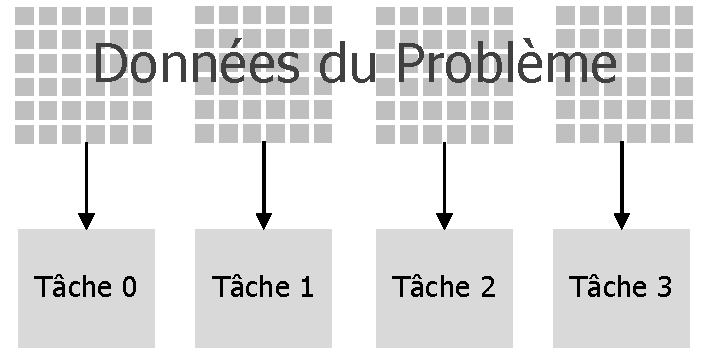
\includegraphics[width=0.8\columnwidth]{Chapter1/figures/domaindecomp}
%	\caption{Partitonnement par d�composition du domaine}
%	\label{figdomain}
%\end{figure}

%Dans ce type de partitionnement, les donn�es associ�es au probl�me sont d�compos�es. Chaque t�che parall�le travaille donc sur une portion des donn�es. Il existe alors plusieurs mani�res de d�composer les donn�es. En traitement d'images, les donn�es sont en 2 dimensions les d�compositions possibles sont illustr�es en figure \ref{decomp2D}.

%\begin{figure}[htb]
%	\centering
%	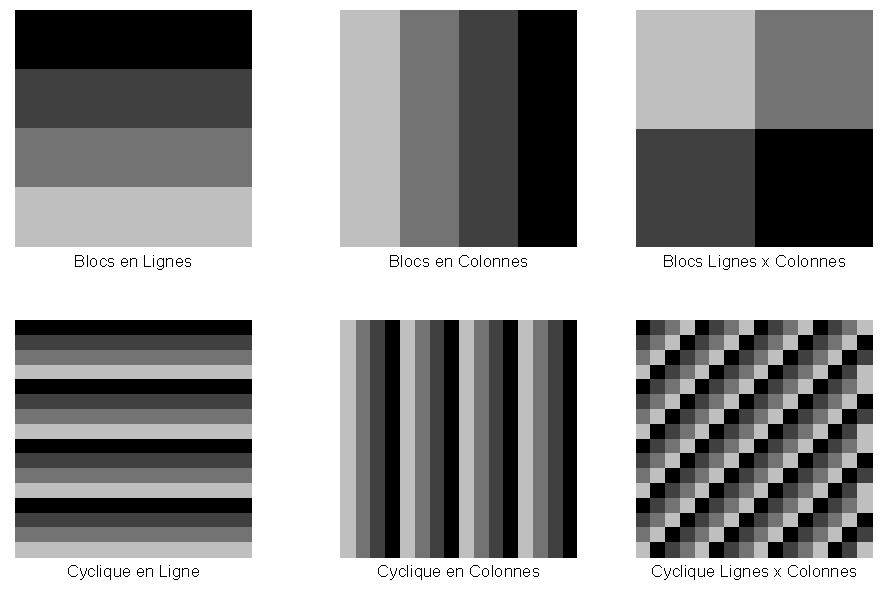
\includegraphics[width=0.8\columnwidth]{Chapter1/figures/decomp2D}
%	\caption{Partitonnement par d�composition du domaine en traitement d'images}
%	\label{decomp2D}
%\end{figure}






\indent Le processeur Cell est une architecture unique en son genre car elle renferme une multitude de dispositifs d�di�s au calcul hautes-performances. Son architecture parall�le � plusieurs niveaux permet aux utilisateurs aguerris d'atteindre des performances jusque l� r�serv�es au cluster de machines et utilisant des paradigmes de hauts niveaux tels que le message-passing. En ce sens l'architecture du Cell destin�e initialement au domaines des jeux vid�os a trouv� d'autres d�bouch�s notamment dans le calcul scientifique au sens large.\\
\indent Le Cell est compos� d'un processeur PowerPC classique nomm� PPE (Power Processor Element) et de huit unit�s de calcul acc�l�ratrices appel�es SPE (Synergestic Processor Element). Cet ensemble d'unit�s de calcul est reli� par un bus interne qui permet aussi l'acc�s � la m�moire principal (Main Storage), ainsi qu'� d'autres p�riph�riques externes. Le processeur Cell est consid�r� comme une architecture h�t�rog�ne car il comporte deux types d'architectures diff�rentes : celle du PPE qui n'est autre qu'une d�clinaison du PowerPC 970 et celle des SPE qui sont des unit�s SIMD acc�l�ratrices sp�cialis�es dans des traitements contenant un flot de donn�e important comme le multim�dia par exemple.\\


\textbf{INSERER FIGURE DU CELL ICI}

\subsubsection{Le PPE:  Power Processor Element}
Le PPE est un processeur 64-bit compatible avec l'architecture Power, optimis� au niveau de l'efficacit� �nerg�tique. La profondeur de pipeline du PPE est de 23 �tages, chiffres qui peut para�tre faible par rapport au pr�c�dentes architectures surtout quand on sait que la dur�e de l'�tage � �t� r�duite d'un facteur 2. Le PPE est une architecture dual-issue (deux instructions peuvent �tre lanc�es par cycle) qui ne reordonance pas dynamiquement les instructions � l'ex�cution (ex�cution dans l'ordre). Le processeur entrelace des instructions provenant de deux threads de calcul diff�rents pour optimiser l'utilisation de la fen�tre d'ex�cution. Les instructions arithm�tiques simples s'ex�cutent et fournissent leur r�sultat en deux cycles. Les instructions de chargements (loads) s'ex�cutent �galement en deux cycles. Une instruction flottante en double pr�cision s'ex�cute en 10 cycles. Le PPE supporte une hi�rarchie conventionnelle de caches avec un cache L1 (de niveau 1) donn�es en instructions de 32-KB, et un cache L2 de 512-KB.\\
Le processeur fournit deux threads d'ex�cution simultan�s et peut �tre vu comme un processeur double-coeur avec un flot de donn�es partag�, ceci donne l'impression au logiciel d'avoir deux unit�s de traitement distinctes. 
Certains registres sont dupliqu�s mais pas les caches qui sont partag�s par les deux threads.\\
Le processeur est compos� de trois unit�s l'unit� d'instructions (UI) responsable du chargement, d�codage, branchements, ex�cution et compl�tion des instructions. Une unit� d'ex�cution des op�rations en arithm�tique point-fixe (XU) qui est �galement responsable des instructions load/store. Et enfin l'unit� VSU qui ex�cute les instructions en virgule flottante ainsi que les instructions vectorielles. Les instructions SIMD dans le PPE sont celle des anciennes g�n�rations de PowerPC 970 et effectuent des op�rations sur des registres 128-bit de donn�es qui donnent un parall�lisme de 2, 4, 8 ou 16, selon le type de donn�es consid�r�.

\subsubsection{Les SPE (Synergistic Processing Element)}
Le SPE contient un jeux d'instructions nouveau mais qui n'est autre qu'une version r�duite du jeux d'instructions SIMD VMX (Altivec), mais qui est optimis�e au niveau de consommation d'�nergie et des performances pour les applications de calcul intensif et de multim�dia. Le SPE contient une m�moire locale de 256 KB (scrathpad) qui est une m�moire de donn�es et d'instructions. Les donn�es et les instructions sont transf�r�es de la m�moire centrale vers cette m�moire priv�e au travers de commande DMA synchrones et coh�rentes qui sont ex�cut�s par le MFC (Memory Flow Controler) qui est pr�sent dans chaque SPE. Chaque SPE peut supporter jusqu'� 16 commandes DMA en suspens. L'unit� DMA peut �tre programm�e de trois mani�res diff�rente: 1) avec des instructions sur le SPE qui ins�rent des commandes DMA dans la file d'attente; 2) Par la programmation de transferts permettant de faire des acc�s sur des zones non contigu�s de la  m�moire au travers d'une liste de DMA; 3) Par l'insertion d'une commande DMA dans la file d'attente d'un autre processeur par les commandes de DMA-write. Afin de faciliter la programmation et de permettre des transferts entre SPEs les m�moire locales sont mapp�es en m�moire centrale. La pr�sence des m�moires locales introduit un autre niveau dans la hi�rarchie m�moire au dessus des registres. Les temps d'acc�s de ces m�moires sont de l'ordre du cycle ce qui en fait de bon candidats pour r�duire la latence d'acc�s � la m�moire centrale qui est de l'ordre de 1000 cycles, d'autant plus que le fait que le contr�leur DMA soit ind�pendant de l'unit� donne un niveau de parall�lisme suppl�mentaire. La pr�sence de ces m�moires priv�es permet diff�rents mod�les de programmation qui peuvent �tre appliqu�s au processeur Cell.

\subsubsection{Le Bus Interne (Element Iterconnect Bus)}
Le bus interne du processeur permet de relier les unit�s de traitement PPE, SPE � la fois entre elles, � la m�moire centrale ainsi qu'� une sortie externe. Le bus contient des chemins de donn�es diff�rents de ceux des requ�tes. Les �l�ments autour du bus sont connect�s par des liaison point-�-point et un arbitre de bus est responsable de la r�ception des commandes et de leur diffusion vers les unit�s. Le bus est constitu� de 4 anneaux d'une largeur de 16-octets deux fonctionnent dans le sens d'une aiguille d'une montre et les deux autres dans le sens inverse. Chaque anneau peux potentiellement g�rer 3 transferts en parall�le si toutefois leurs chemins ne se croisent pas. Le EIB op�re � une fr�quence qui est la moiti� de celle du processeur, chaque unit� du bus peut simultan�ment envoyer et recevoir 16 octets par cycle d'horloge du bus.
\chapter{Mod�les de Programmation}
Dans ce chapitre on se propose de faire une revue des mod�les de programmation pour le processeur Cell. Par mod�le de programmation on entend outils de d�ploiement de code ou de parall�lisation con�us pour le Cell. Les approches cit�es dans ce qui suit sont celles qui nous ont paru pertinents et assez mures pour pouvoir �tre utilis�es dans notre domaine d'applications. Certaines approches reprennent des outils existants pour les architectures parall�les � m�moire partag�e ou distribu�e qui ont �t� adapt�s pour l'architecture et la hi�rarchie m�moire du Cell.
%====================================================== THREADS POSIX ======================================================================================================================================
\section{Les Threads POSIX}
Les threads POSIX\footnote{Portable Operating System Interface for Unix} ou \emph {Pthreads} sont une standardisation\cite{pthreads_std} du mod�le de programmation par threads pour les syst�mes UNIX. Ce mod�le est bas� sur une API de programmation parall�le qui permet la gestion des threads ainsi que la synchronisation par mutex ou variables conditionnelles. Historiquement, les concepteur de hardware ont d�velopp� leurs impl�mentations propri�taires des threads, ceci a rendu la portabilit� du code des programmeurs quasi impossible. La n�cessit� d'une API standard est donc devenue vitale, c'est pour cette raison que la majorit� des vendeurs de hardware poss�dent actuellement leur impl�mentation  standard des threads POSIX. Les Pthreads sont d�finis autour d'un ensemble de proc�dures et de types en langage C contenus dans le fichier d'ent�te \texttt{"pthread.h"}.\\
D'une mani�re g�n�rale un thread est un flux d'instructions pouvant s'ex�cuter de mani�re ind�pendante sur un OS donn�. Du point de vue du programmeur ceci s'apparente � une procedure qui peut s'ex�cuter ind�pendamment du programme principal, un programme contenant des proc�dures de ce type est dit \emph{multi-threaded}. Afin de d�tailler le principe de fonctionnement des threads il est n�cessaire de faire un rappel sur les \emph{process} UNIX. Un \emph{process} est cr�� par l'OS est contient un certain overhead qui consiste en certaines ressources n�cessaires � son ex�cution. Les threads r�sident � l'int�rieur de ces ressources et sont capables d'�tre ordonnanc�s et ex�cut�s en tant qu'entit�s ind�pendantes car ils ne dupliquent qu'une partie des ressources qui leurs permettent d'�tre des morceaux de code ex�cutables. Le flot de contr�le est rendu ind�pendant car le thread poss�de ses propres: pointeur de pile, registres, propri�t�s d'ordonnancement (priorit� et politique), ensemble de signaux et donn�es sp�cifiques. En somme, un thread existe dans un process dont il utilise les ressources. Il poss�de son propre flot de contr�le et ne duplique que les ressources n�cessaires � son ex�cution ind�pendante. Il peut partager les ressources du process avec d'autres threads et s'ex�cuter en coordination avec ces derniers. La complexit� due � sa cr�ation et � sa gestion est l�g�re comparativement � celle du process et sa dur�e de vie est celle de son process parent.
\subsection{l'API Pthread}
L'API des threads POSIX peut �tre d�compos�e en trois types de routines:
\begin{itemize}
\item \textbf{Les routines de gestion des threads} : comprends les t�ches de cr�ation, propri�t�s d'ex�cution et terminaison des threads.
\item \textbf{Les \emph{mutex}} (abbreviation de \emph{mutual exclusion}): ils permettent de synchroniser les threads, les routines g�rent la cr�ation, destruction, r�servation et lib�ration des \emph{mutex}.
\item \textbf{Les variables conditionnelles} : ces derni�res g�rent la communication entre des threads qui partagent les \emph{mutex}. Elles sont bas�es sur des conditions fix�es par le programmeur, elles incluent des fonctions de cr�ation, destruction, attente et signalisation bas�es sur certaines valeurs de ces variables. 
\end{itemize}
\rule{\textwidth}{0.2mm}\\
\subsubsection{Gestion des Threads}
\begin{itemize}
\item \textbf{Cr�ation et Terminaison des Threads}: Initialement le programme contient un seul thread qui est le \texttt{main()}. Les autres threads doivent �tre cr��s explicitement par le programmeur. \texttt{pthread\_create} cr�� un nouveau thread et le rend ex�cutable, un exemple de code � base de \emph{Pthreads} est donn� dans le listing \ref{pthreadcode}. Cette routine peut �tre appel�e autant de fois que l'on veut et � n'importe quel endroit dans le code. Le nombre de threads maximal cr�� par un process d�pend de l'impl�mentation. Une fois cr��s les threads peuvent cr�er � leur tour d'autres threads et il n'existe aucune d�pendance ni hi�rarchie entre les threads. Le thread est cr�e avec certains attributs par d�faut, ceux-ci pouvant �tre chang�s ult�rieurement. Il existe plusieurs mani�res de terminer un thread: soit par le thread lui m�me qui le fait par un return de sa routine principale ou par la fonction \texttt{pthread\_exit()}, ou alors par un autre thread en utilisant \texttt{pthread\_cancel()} et enfin en cas de terminaison du process parent.
\item \textbf{Passage d'Arguments au Threads} : On peut passer un argument au thread via la routine \texttt{pthread\_create()}. On peut �galement passer plusieurs arguments en les rassemblant dans une structure et en passant l'adresse de celle-ci.
\item \textbf{Jonction et D�tachement des Threads} : La jonction est une mani�re de faire une synchronisation entre les threads, la fonction \texttt{pthread\_join()} bloque le thread appelant jusqu'a ce que le thread appel� termine son ex�cution. Le caract�re joignable ou pas d'un thread est sp�cifi� � sa cr�ation : s'il est cr�e en tant que thread d�tach� il ne pourra pas �tre joignable. La routine \texttt{pthread\_detach()} sert � d�tacher un thread qui �tait joignable � sa cr�ation.
\item \textbf{Gestion de la Pile} : Le standard ne d�finit pas la taille par d�faut de la pile du thread, celle-ci d�pend de l'impl�mentation. Toutefois, le programmeur peut en sp�cifier la taille ainsi que l'emplacement de la m�moire dans laquelle elle doit �tre stock�e.
\end{itemize}

\subsubsection{Les Variables \emph{mutex}}
Les \emph{mutex} sont un des principaux m�canismes de synchronisation de threads. Ils permettent par exemple de synchroniser des threads ou alors de prot�ger des donn�es partag�es en cas d'�criture simultan�e. Un \emph{mutex} peut �tre r�serv� (\emph{lock}) par un seul thread � un moment donn�, le propri�taire du \emph{mutex} est le seul � le poss�der : tout autre thread qui essaye de r�server ce m�me \emph{mutex} �choue jusqu'� ce que le propri�taire le lib�re (\emph{unlock}). Il existe des routines de cr�ation et de destruction des \emph{mutex}, la r�servation des \emph{mutex} se fait soit par appel � la routine \texttt{pthread\_\emph{mutex}\_lock()} (bloquant), \texttt{pthread\_\emph{mutex}\_trylock()} (non bloquant) et se lib�re par \texttt{pthread\_\emph{mutex}\_unlock()}. Parmi les exemples d'utilisation des \emph{mutex} on peut citer les cas de \emph{race condition} o� plusieurs threads essayent de mettre � jour une variable globale, il est n�cessaire dans ce genre de situations de prot�ger cette variable par un \emph{mutex} afin que celle-ci ait la m�me valeur du point de vue de tous les threads. On dit alors que l'on cr�e une \emph{section critique}.
%===============================Listing Pthreads =======================================
\lstset{ %
language=C,                % choose the language of the code
basicstyle=\footnotesize,       % the size of the fonts that are used for the code
backgroundcolor=\color{light-gray},  % choose the background color. You must add \usepackage{color}
showspaces=false,               % show spaces adding particular underscores
showstringspaces=false,         % underline spaces within strings
showtabs=false,                 % show tabs within strings adding particular underscores
frame=single,			% adds a frame around the code
tabsize=2,			% sets default tabsize to 2 spaces
captionpos=b,			% sets the caption-position to bottom
breaklines=true,		% sets automatic line breaking
breakatwhitespace=false,	% sets if automatic breaks should only happen at whitespace
escapeinside={\%*}{*)}  ,        % if you want to add a comment within your code
caption = Exemple de code \emph{Pthread} basique montrant les routines de cr�ation de \emph{threads},
label = pthreadcode
}
\lstinputlisting{Chapter1/Code/pthreadexample.c}
%===================================================================================
\subsubsection{Les Variables de Condition}
Les variables de condition fournissent aux threads une autre mani�re de se synchroniser. Contrairement aux \emph{mutex} qui sont bas�s sur le contr�le de l'acc�s � une variable, la synchronisation par variable de condition se fait selon une valeur sp�cifi�e. Les variables de condition sont utilis�es en conjonction avec les \emph{mutex}. L'appel � la fonction \texttt{pthread\_cond\_wait()} bloque le thread appelant jusqu'� ce que la condition sp�cifi�e est signal�e. Cette routine doit �tre appel�e tant que le \emph{mutex} est r�serv� et lib�re automatiquement le \emph{mutex} quand elle est en attente. Une fois que le signal est re�u, le thread est r�veill� et le \emph{mutex} est r�serv� automatiquement pour �tre utilis� par le thread. La responsabilit� de lib�rer le \emph{mutex} est � la charge du programmeur qui le fait une fois que son utilisation n'est plus n�cessaire. La fonction \texttt{pthread\_cond\_signal()} est utilis�e pour signaler (ou r�veiller) un autre thread qui est en attente de la variable de condition. Elle doit �tre appel� apr�s que le \emph{mutex} est r�serv� et doit lib�rer le \emph{mutex} dans l'ordre pour permettre � \texttt{pthread\_cond\_wait()} de s'achever. Il existe une routine nomm�e \texttt{pthread\_cond\_broadcast()} qui met en attente plusieurs threads en m�me temps. 


\subsection{Les Threads POSIX sur le Cell}
Sur un syst�me Linux pour le Cell, the thread principal s'ex�cute sur le PPE, celui-ci pouvant produire un ou plusieurs t�ches sur le processeur. Une t�che peut contenir un ou plusieurs threads Linux qui peuvent s'ex�cuter soit sur le PPE soit sur le SPE. Un thread qui s'ex�cute sur le SPE poss�de son propre contexte incluant un banc de registre de 128 x 128-bit  , un compteur de programme et une file d'attente de commandes MFC, et il peut communiquer avec d'autres unit�s d'ex�cution au travers de l'interface des canaux MFC. Un thread PPE peut interagir directement avec un thread SPE via sa m�moire locale ou son espace de \emph{problem state} ou indirectement via la m�moire centrale ou les routines la \emph{SPE Runtime Management Library}. L'OS d�finit le m�canisme et la politique d'ordonnancement pour les SPE disponibles, il est �galement responsable de la gestion des priorit�s entre les t�ches, du chargement du programme de la notification des �venemments au SPEs ainsi que du support du debugger.
Une API de gestion des threads SPE similaire � la librairie POSIX a �t� con�ue, dans le but de fournir � la fois un environnement de programmation familier et une flexibilit� dans la gestion des SPEs. Cette API supporte � la fois la creation et la terminaison des t�ches SPE ainsi que l'exclusion mutuelle par des primitives de mise � jour atomiques. L'API peut acc�der au SPE en utilisant un mod�le virtuel dans lequel l'OS affecte dynamiquement les threads aux SPEs dans l'ordre de leur disponibilit�. Les applications, peuvent sp�cifier de mani�re optionnelle un masque d'affinit�s pour affecter les threads a un SPE sp�cifique. Les dispositifs architecturaux de communication entre les threads et de synchronisation (mailbox, signaux, etc...) peuvent �tre acc�d�s via un ensemble d'appels syst�me ou alors via l'application qui mappe un block de contr�le du SPE dans l'espace m�moire de l'application. Sur le Cell il existe trois blocks de contr�le du SPE, un acc�d� par l'application, un autre par l'OS et un troisi�me par un superviseur. Une interface accessible � l'utilisateur permet  la communication directe entre les processeurs SPEs ou PPE, ceci permet d'�viter des appels syst�me co�teux.\\
Lorsque l'application fait une requ�te de creation de threads, la librairie de threads SPE envoie la requ�te � l'OS pour alouer un SPE et cr�er un thread SPE � partir d'un fichier objet de format ELF (Executable and Linkable Format) int�gr�e dans un executable Cell. Le \emph{miniloader} un programme SPE de 256-bit, t�l�charge la segment de code � ex�cuter sur le SPE, l'avantage de cette approche et d'une part d'�viter au PPE d'effectuer cette t�che et d'autre part de profiter du fait que les les transfers PPE-SPE quand il se font du c�t� SPE, sont nettement plus efficace grace � une interface qui contient plus de canaux de communications.
\begin{figure}[!htbf]
	\centering
	\includegraphics[scale =0.6]{Chapter1/Figures/cell_compilation_process}
	\caption{Processus \emph{dual source} de g�n�ration de code ex�cutable pour le Cell}
  \label{seq_fig1}
\end{figure}
\subsection{Processus de G�n�ration de Code}
Dans le mod�le de programmation d�crit ci-dessus le processus de g�n�ration de code binaire ex�cutable sur le Cell est dit \emph{dual-source}. En effet, il existe deux code sources distincts, un code pour le SPE (spe.c sur la figure \ref{fig_comppocess})) qui contient le code ex�cut� sur le SPE. Un deuxi�me code source qui est celui s'ex�cutant sur le PPE contient le \emph{thread} ma�tre qui g�re les \emph{threads} SPE. Le processus de g�n�ration de code ex�cutable est d�crit dans la figure \ref{fig_comppocess}. Dans la premi�re �tape le code SPE est compil� ce qui donne un binaire ex�cutable SPE. Celui-ci est par la suite trait� par un outils sp�cifique \emph{spu-embedd} qui permet de transformer ce binaire en bout de code qui peut �tre enfouis dans l'ex�cutable du PPE. Cette proc�dure se fait par l'outil d'�dition de lien qui consid�re alors le code SPE comme une librairie dont le code objet doit �tre int�gr� dans l'ex�cutable final.
\subsection{conclusion}
La programmation par threads sur le Cell est le mod�le de base pour la mise en ouvre de code parall�le sur cette architecture. Il est caract�ris� par une API tr�s bas niveau qui permet en m�me temps de garder un contr�le pr�cis sur le d�roulement de son application et d'avoir une grande fl�xibilit� en terme de choix de d�ploiement d'un algorithme donn�. Gr�ce au dispositifs architecturaux de signalisation et de synchronisation, l'interface est rendue tr�s efficace en terme de performance sur le Cell. Toutefois, du point de vue du programmeur, la mise en oeuvre du code est s�rement plus laborieuse que pour d'autres mod�les de programmation, mais celle-ci peut �tre justifi�e dans le cadre de fortes contraintes sur les temps d'ex�cution ou dans le cas ou le mod�le de calcul SPMD n'est pas adapt� � l'application d�ploy�e. 

%====================================================== RAPIDMIND ======================================================================================================================================

\section{RapidMind}
\textbf{RapidMind}\cite{rapidmind} est un mod�le de programmation parall�le multi-plateformes, GPU, multi-coeur sym�trique et pour le processeur Cell, il rel�ve du mod�le de programmation \emph{stream programming} et s'apparente � un langage de programmation enfoui dans C++. Il est bas� sur la biblioth�que template C++ et une librairie de runtime qui effectue la g�n�ration dynamique de code. La librairie template permet l'invocation de code SPE � l'int�rieur du code PPE, avec l'ensemble du code SPE �crit en template.\\
La librairie template de \textbf{RapidMind} fournit un ensemble de types de donn�es, des macros de contr�le, des op�rations de r�duction et des  fonctions communes qui permettent � la librairie de runtime de capturer une repr�sentation du code SPE (retained code). Les types de donn�es ont �t� sp�cialement con�us pour exprimer de mani�re simple les op�rations SIMD et les exposer facilement � la librairie runtime. Le runtime � son tour extraits le parall�lisme � partir de ces op�rations  en vectorisant le code et en divisant les calculs sur les tableaux et les vecteurs sur les diff�rents SPEs. Il peut �galement effectuer des optimisations de boucle comme les d�tection des invariants de boucle. \textbf{RapidMind} assigne des t�ches aux SPEs dynamiquement et peut effectuer des optimisations � plus haut niveau comme la superposition des calculs et des transferts qui permet de masquer la latence de ces derniers. Enfin, le mod�le de calcul est un mod�le SPMD, il diff�re du mod�le SIMD du fait que les programme peuvent contenir du flot de contr�le et par le fait que celui-ci puisse g�rer une certaine forme de parall�lisme de t�ches m�me si �tant initialement un mod�le \emph{data-parallel}. Un exemple de code \emph{RapidMind} est donn� dans le listing \emph{rapidmindcode}.\\
\subsection{Mod�le de Programmation et Interface}
L'interface est bas�e sur trois types C++ principaux: \textbf{\texttt{Value<N,T>}}, \textbf{\texttt{Array<D,T>}} et \textbf{\texttt{Program}}, tous sont des conteneurs, les deux premiers pour les donn�es et le dernier pour les op�rations. Le calcul parall�le est effectu� soit en applicant des \textbf{\texttt{Program}} sur des \textbf{\texttt{Array}} pour cr�er de nouveaux \textbf{\texttt{Array}}, ou en applicant une op�ration collective parall�le qui peut �tre param�tr�e par un objet \textbf{\texttt{Program}} comme la r�duction par exemple.\\
A premi�re vue, les types \textbf{\texttt{Value}} et \textbf{\texttt{Array}} ne sont pas une grande nouveaut�. En effet, tout d�veloppeur C++ a pour habitude d'utiliser les types N-tuples pour exprimer le calcul num�rique sur des vecteurs, et le type \textbf{\texttt{Array}} est une mani�re usuelle d'encapsuler la v�rification des valeurs limites (boundary checking). Toutefois ces types constituent une interface pour une machine parall�le puissante bas�e sur la g�n�ration dynamique de code. Ceci est rendu possible gr�ce au type \textbf{\texttt{Program}} qui est la principale innovation du mod�le de programmation \textbf{RapidMind}. Un mode d'ex�cution symbolique \emph{retained} est utiliser pour collecter dynamiquement des op�rations arbitraires sur les \textbf{\texttt{Value}} et les \textbf{\texttt{Array}} dans les objets \textbf{\texttt{Program}}.
\subsubsection{le type \textbf{\texttt{Value}}}
le type \textbf{\texttt{Value<N,T>}} est un N-tuple, les instances de ce type contiennent N valeurs de type T, ou T peut �tre un type num�rique de base (un flottant simple ou double pr�cision ou tout autre type entier), les flottants 16-bits sont �galement support�s. Des notations courtes existent pour certaines tailles usuelle comme le \textbf{\texttt{Value4f}} pour un quartet de floats ou \textbf{\texttt{Value3ub}} pour un triplet d'entiers 8-bits non sign�s.\\
Les op�rations arithm�tiques standard et les op�rations logiques sont surcharg�s pour les types tuples et op�rent composante par composante. Les fonctions de la biblioth�que standard  sont �galement support�es, comme les fonctions trigonom�triques et logarithmiques. En plus des op�rations arithm�tiques, des op�rations de r�organisation des donn�es on �t� ajout�es au type value: ces op�rations permettent la duplication d'une composante ou ou le permutation des composantes. Par exemple, si \textbf{\texttt{a}} est une valeur de type \textbf{\texttt{Value<4, float>}} qui repr�sente une couleur RGBA, a(2,1,0) est l'inverse repr�sentant le triplet BGR.\\
Les calculs sont exprim�s en utilisant les tuples de \textbf{\texttt{Value}} et les op�rateurs sur ces types peuvent �tre utilis�s directement pour exprimer du parall�lisme SWAR (SIMD Within A Register). \subsubsection{le type \textbf{\texttt{Array}}}
Le type \textbf{\texttt{Array<D,T>}} est �galement un conteneur de donn�es. Ce qui le distingue du type \textbf{\texttt{Value}} est le fait qu'il peut avoir plusieurs dimensions et que sa taille est variable. L'entier D repr�sente la dimensionnalit� (1,2 ou 3), le type T est le type des �l�ments du conteneur. Le type des �l�ments et pour le moment restreint aux instances du type \textbf{\texttt{Value<N,T>}}.\\
Les instances du type \textbf{\texttt{Array}} supportent les op�rateurs "[]" et "()" pour l'acc�s al�atoire aux donn�es. L'op�rateur "[]" utilise des entiers en arguments tandis que l'op�rateur "()" utilise des coordonn�es r�elles comprises dans [0, 1] dans chaque dimension, cette particularit� est utile par exemple pour les modes d'interpolation des images.\\
Les sous-tableaux peuvent �tre acc�d�s en utilisant les fonctions \textbf{slice}, \textbf{offset} et \textbf{stride}. Les effets de bords sont g�r�s en utilisant la fonction membre \textbf{boundary}, qui inclut diff�rents modes de traitement pour les bords. les types \textbf{\texttt{Value}} et \textbf{\texttt{Array}} suivent une s�mantique par valeurs qui permet d'�viter l'aliasing de pointeurs et simplifie la programmation et l'optimisation. Il existe �galement d'autres types de sous-tableaux, les r�f�rences sur tableaux et les accesseurs.
\subsubsection{le type \textbf{\texttt{Program}}}
Un objet \textbf{\texttt{Program}} contient une s�quence d'op�rations, ces op�rations sont sp�cifi�es par le passage en mode \emph{retained} qui est indiqu� par la macro mot-cl� \textbf{\texttt{BEGIN}}. Normalement, le syst�me fonctionne en mode \emph{immediate}. Dans ce mode les op�rations sur un tuple de valeurs s'ex�cutent � la sp�cification comme pour une biblioth�que matrice-vecteur classique:  les calculs sont effectu�s sur la m�me machine que le programme h�te et le r�sultat est sauvegard� dans le tuple \textbf{\texttt{Value}} de sortie. En mode \emph{retained} un nouvel objet \textbf{\texttt{Program}} qui est retourn� par la macro \textbf{\texttt{BEGIN}} est cr�e. Les op�rations dans ce mode ne sont pas ex�cut�es; elles sont symboliquement �valu�es et sauvegard�es dans l'objet \textbf{\texttt{Program}}. La sortie du mode \emph{retained} est marqu�e par la macro \textbf{\texttt{END}}, qui ferme l'objet \textbf{\texttt{Program}} et le marque comme �tant pr�t � �tre compil�, �tape � la suite de laquelle l'objet \textbf{\texttt{Program}} est utilis� pour le calcul. Les objets \textbf{\texttt{Program}} sont compil�s de mani�re dynamique ce qui permet d'exploiter les caract�ristiques bas-niveau de la machine cible.\\
Il est � noter que m�me si les types \textbf{RapidMind} sont des classes C++, le compilateur est plut�t assimilable � un compilateur FORTRAN et peut ainsi effectuer les m�mes optimisations agressives. Les fonctionnalit�s du langage C++ sont utilis�es pour structurer les calculs et g�n�rer le code mais pas lors de l'ex�cution.
\subsection{Evaluation Partielle et Alg�bre du Programme}
Les objets \textbf{\texttt{Program}} sont des conteneurs d'op�rations, et ces op�rations peuvent �tre manipul�es par le syst�me de mani�re explicite. Cela permet l'impl�mentation de plusieurs dispositifs avanc�s de programmation.\\\\
%===============================Listing Rapidmind =======================================
\lstset{ %
language=C,                % choose the language of the code
basicstyle=\footnotesize,       % the size of the fonts that are used for the code
backgroundcolor=\color{light-gray},  % choose the background color. You must add \usepackage{color}
showspaces=false,               % show spaces adding particular underscores
showstringspaces=false,         % underline spaces within strings
showtabs=false,                 % show tabs within strings adding particular underscores
frame=single,			% adds a frame around the code
tabsize=2,			% sets default tabsize to 2 spaces
captionpos=b,			% sets the caption-position to bottom
breaklines=true,		% sets automatic line breaking
breakatwhitespace=false,	% sets if automatic breaks should only happen at whitespace
escapeinside={\%*}{*)}  ,        % if you want to add a comment within your code
caption = Exemple de parall�lisation de code avec \emph{RapidMind},
label = rapidmindcode
}
\lstinputlisting{Chapter1/Code/rapidmindexample.c}
En premier lieu, les \textbf{\texttt{Program}} peuvent �tre �valu�s partiellement. Si un objet \textbf{\texttt{Program}} \textbf{p} ayant \textbf{n} entr�es, l'expression \textbf{p(A)} retourne un objet \textbf{\texttt{Program}} avec \textbf{(n-1)} entr�es. En d'autres termes les entr�es de l'objet \textbf{\texttt{Program}} ne sont pas obligatoirement fournies en une fois. Il est possible de binder toutes les entr�s d'un objet \textbf{\texttt{Program}} mais de diff�rer son ex�cution effective. L'ex�cution d'un objet \textbf{\texttt{Program}} n'est d�clench�e que quand il est affect� � un \emph{bundle}, \textbf{\texttt{Array}} ou \textbf{\texttt{Value}}. L'op�rateur \textbf{"()"} est utilis� pour binder les entr�es de l'objet \textbf{\texttt{Program}}. Ceci est appel� le \emph{tight binding}. Un changement de l'entr�e apr�s un \emph{tight binding}, n'affecte pas les entr�es d'un \textbf{\texttt{Program}}, m�me si son ex�cution est diff�r�e. Dans l'exemple pr�c�dent, ou l'on cr�e \textbf{"p(A)"} et on l'affect � un objet \textbf{\texttt{Program}} \textbf{"q"}, et qu'on modifie ensuite l'entr�e \textbf{"A"}. Lors de l'ex�cution de \textbf{"q"}, celui-ci utilisera la valeur de \textbf{"A"} au moment du binding dans \textbf{"p"}, pas la valeur modifi�e. Le \emph{tight binding} permet l'optimisation de l'objet \textbf{\texttt{Program}} bas�e sur les valeurs effectives dans l'entr�e bind�e.\\
Toutefois, le syst�me supporte �galement le \emph{loose binding}, sp�cifi� par l'op�rateur \textbf{"<<"}. L'expression \textbf{"p<<A"} est similaire � \textbf{"p(A)"} sauf que les changements sur \textbf{"A"} sont visibles � l'ex�cution diff�r�e de \textbf{"p<<A"}.\\
%===================================================================================
Une entr�e � un \textbf{\texttt{Program}} peut �tre bind�e � un \textbf{\texttt{Array}} ou un tuple de \textbf{\texttt{Value}}. Si des arrays de tailles diff�rentes sont bind�es � un \textbf{\texttt{Program}} la plus petite entr�e est r�pliqu�e suivant les conditions aux bords pour avoir la taille de l'entr�e de l'entr�e la plus grande.\\
Les \textbf{\texttt{Program}} peuvent �tre combin�s pour cr�er de nouveaux \textbf{\texttt{Program}} en utilisant deux op�rations: la composition fonctionnelle est le \emph{bundling}. Ces op�rations forment une alg�bre ferm�e dans l'ensemble des objets \textbf{\texttt{Program}}. L'op�rateur de composition fonctionnelle \textbf("<<") quand il est appliqu� � deux objets \textbf{\texttt{Program}} \textbf{"p"} et \textbf{"q"} \textbf{"p << q"} transmet toutes les entr�es du \textbf{\texttt{Program}} � droite de l'op�rateur � l'entr�e de celui de gauche, il cr�e un nouvel objet \textbf{\texttt{Program}} ayant les entr�es de \textbf{"q"} et les sorties de \textbf{"p"}. L'op�rateur \emph{bundle} quand � lui utilise la fonction \textbf{"bundle"}. Cette fonction concat�ne toutes les entr�es/sorties de ses arguments dans l'ordre et cr�e un nouvel objet \textbf{\texttt{Program}} �quivalent � la concat�nation des sources de ces \textbf{\texttt{Program}} d'entr�e en s�quence.\\
Ces op�rations combin�es avec la compilation dynamique permettent une am�lioration consid�rable des performances surtout quand le programme est domin� par des instructions de m�moire.

\subsection{Les Op�rations Collectives}
L'op�ration de base support�e est l'application parall�le d'un programme sur un tableau de donn�es. Toutefois, d'autres patterns de communication et de calcul sont support�s sous la forme d'op�rations collectives. Les patterns de communication irr�guliers sont fournis par les op�rations de \emph{scatter} et \emph{gather},et l'op�ration de r�duction fournit un pattern de calcul hi�rarchique.\\
L'op�ration\emph{gather} permet de r�cup�rer des donn�es r�sidant dans des emplacements non-contigus de la m�moire et l'op�ration \emph{scatter} l'�criture dans des zones de m�me nature. L'op�ration de r�duction quand � elle est programmable, elle prend deux entr�e et fournit une sortie. Elle permet par exemple de sommer les �l�ments d'un vecteur d'une mani�re hi�rarchique.\\ \textbf{INSERER FIGURE REDUCTION}\\. On pourra noter que l'op�rateur impliqu� dans la r�duction doit �tre associatif. Parmi les op�rateurs qui ont �t� impl�ment�s on peut citer \textbf{sum}, \textbf{product}, \textbf{min} et \textbf{max}.
\subsection{Sp�cificit� du Backend pour le Cell de RapidMind}
L'impl�mentation de RapidMind pour le Cell poss�de certaines particularit�s qui tiennent compte de l'architecture particuli�re de ce processeur. Le parall�lisme SWAR peut �tre mapp� directement sur les registres SIMD du SPE mais les op�rations de permutation de donn�es ne sont pas impl�ment�es de mani�re aussi efficace les unes que les autres. D'autre part la parall�lisation qui consiste � appliquer un program � un tableau permet en th�orie de faire des millions de calculs en parall�le, mais le Cell ne poss�de qu'un nombre limit� d'unit�s de traitement. C'est pour cela que les donn�es sont subdivis�e en plusieurs paquets et transf�r�es dans les m�moires locales des SPEs avant d'�tre trait�es. Le triple buffering est utilis� pour cacher la latence des transferts DMA. Pour les acc�s m�moire non r�guliers un software-cache est utilis�. Si les programmes incluent un flux de contr�le, des t�ches diff�rentes peuvent prendre des temps d'ex�cution diff�rents et un syst�me de \emph{load balancing} (�quilibrage de charge) est mis en place. 
\subsection{Conclusion}
La plate-forme de d�veloppement RapidMind combine une interface bas�e sur la compilation dynamique et un mod�le de calcul data-parallel. Elle peut �tre consid�r�e soit comme une API de calcul parall�le ou un langage de programmation parall�le enfoui dans C++. Elle supporte plusieurs niveaux de parall�lisme notamment le parall�lisme SWAR et le parall�lisme SPMD. Le mod�le de programmation est commun � plusieurs plate-formes GPU, multi-coeur et Cell. C'est un mod�le de programmation assez simple � utiliser et qui repose en grande partie sur un compilateur C++ ce qui lui conf�re une grande popularit� aupr�s des utilisateurs. Au niveau des performances on peut relever de bon r�sultats dans \cite{rapidmind} mais pour ce qui est de notre domaine d'applications qui est le traitement d'images, une analyse approfondie sera faite par la suite.

%====================================================== OPENMP ======================================================================================================================================
\section{OpenMP}
OpenMP pour le Cell\cite{cell_omp} int�gr� dans le compilateur XL d'IBM est bas� sur les transformations du compilateur et une librairie de runtime. Le compilateur transforme des pragmas OpenMP en code source interm�diaire qui impl�mente les constructions OpenMP correspondantes. Ce code inclut des appels aux fonctions de la a la librairie de runtime du Cell. Cette derni�re fournit des fonctionnalit�s basiques � OpenMP incluant la gestion des threads, la r�partition de la charge de travail ainsi que la synchronisation. Un exemple de parall�lisation d'une boucle for est donn� dans le listing \ref{ompexample}.\\
Chaque segment de code compris dans une construction parall�le est list� par le compilateur dans une fonction s�par�e. Le compilateur ins�re les appels � la librairie de runtime OpenMP dans la fonction parente de la fonction list�e. Ces appels aux fonctions de la librairie de runtime vont ainsi invoquer les fonction list�es et g�rer leur ex�cution.\\
Le framework est bas� sur le compilateur IBM XL. Ce dernier poss�de des front-end pour C/C++ et FORTRAN, et contient la m�me infrastructure d'optimisation pour ces langages. Le framework d'optimisation se divise en deux composants TPO et TOBEY. TPO est charg� des optimisations haut niveau ind�pendantes de la machine cible tandis que TOBEY effectue les optimisations bas-niveau sp�cifiques � l'architecture.\\
Le compilateur r�sulte d'une adaptation de versions existantes du compilateur XL supportant OpenMP, mais la sp�cificit� de l'architecture du Cell � pos� quelques probl�matiques qui sont les suivantes:
\begin{itemize}
\item \textbf{Threads et Synchronisation}: les threads s'ex�cutant sur le PPE diff�rent de ceux du SPE en termes de capacit� de traitement. Le syst�me � �t� con�u pour prendre en compte la diff�rence entre les deux architectures.
\item \textbf{G�n�ration de Code}: Le jeu d'instruction du PPE diff�re de celui du SPE. Il en r�sulte que l'optimisation du code PPE est faite s�par�ment de celle du SPE. L'espace de stockage sur le SPE �tant limit�, le code SPE s'il exc�de cette capacit�, peut �tre partitionn� en sections binaires (\emph{overlays}) au lieu d'une section monolithique. De plus, les donn�es partag�es dans le code SPE n�cessitent un transfert DMA de la m�moire centrale vers la m�moire locale. Ceci est fait soit par le compilateur qui ins�re explicitement des commandes DMA dans le code, soit par un m�canisme de software cache qui fait partie de la librairie de runtime du SPE.\\
\item \textbf{Mod�le M�moire}: le hardware du Cell assure que les transactions DMA sont coh�rents, mais ne fournit pas de m�canisme de coh�rence pour les donn�es r�sidant dans la m�moire locale, le mod�le m�moire de OpenMP impl�ment� assure une coh�rence de donn�es qui est requise par les sp�cifications.
\end{itemize}
%===============================Listing OMP =======================================
\lstset{ %
language=C,                % choose the language of the code
basicstyle=\footnotesize,       % the size of the fonts that are used for the code
backgroundcolor=\color{light-gray},  % choose the background color. You must add \usepackage{color}
showspaces=false,               % show spaces adding particular underscores
showstringspaces=false,         % underline spaces within strings
showtabs=false,                 % show tabs within strings adding particular underscores
frame=single,			% adds a frame around the code
tabsize=2,			% sets default tabsize to 2 spaces
captionpos=b,			% sets the caption-position to bottom
breaklines=true,		% sets automatic line breaking
breakatwhitespace=false,	% sets if automatic breaks should only happen at whitespace
escapeinside={\%*}{*)}  ,        % if you want to add a comment within your code
caption = Exemple de code \emph{OpenMP} o� une  boucle for est parall�lis�e,
label = ompexample
}
\lstinputlisting{Chapter1/Code/ompexample.c}
%===================================================================================
Les sections qui suivent d�crivent la mani�re avec laquelle ces probl�mes ont �t� trait�s.
\subsection{Threads et Synchronisation}
les threads peuvent s'ex�cuter sur le PPE ou les SPE. Le thread ma�tre est toujours ex�cut� sur le PPE. Celui-ci est responsable de la cr�ation des autres threads, de la r�partition et de l'ordonnancement des t�ches, et des op�rations de synchronisation. L'absence d'OS sur le SPE fait que le PPE g�re toutes les requ�tes OS. Cette r�partition permet au SPE de se consacrer uniquement aux t�ches de calcul.\\
Actuellement, un seul thread est sens� s'ex�cuter sur le PPE, est le nombre de threads parall�les ex�cut�s sur les SPEs se d�clare par la variable d'environnement OMP\_NUM\_THREADS. La cr�ation et synchronisation des threads est impl�ment�e les librairies du SDK (Software Development Kit). Le thread sur le PPE cr�e des threads SPE au runtime seulement quand les structures parall�les sont rencontr�es pour la premi�re fois.\\
Pour les niveaux de parall�lisme nich�s (boucles nich�es), chaque thread dans la region parall�le la plus externe ex�cute s�quentiellement la r�gion parall�le interne. les it�rations de boucles sont divis�es en autant de morceaux qu'il y a de threads, avec un m�canisme d'ordonnancement et de synchronisation simplifi�. Lorsque le thread SPE est cr�e, il effectue des initialisations et entre dans une phase d'attente d'affectation de t�ches de la part du PPE, ex�cute ces t�ches et se met en attente d'autres t�ches, jusqu'� ce qu'il re�oive un signal de fin de t�ches. Une t�che SPE peut �tre l'ex�cution d'une region parall�le list�e (boucle ou section), ou alors l'ex�cution d'un flush de cache ou encore la participation � une op�ration de synchronisation par barri�re.\\
Il existe une file d'attente dans la m�moire syst�me correspondant � chaque thread. Quand le thread ma�tre assigne une t�che � un thread SPE, il �crit les informations sur cette t�che sur la file d'attente qui lui est consacr�e, incluant le type de t�che, les bornes sup�rieure et inf�rieure de la boucle parall�le, ainsi que le pointeur de fonction pour la r�gion de code list�e qui doit �tre ex�cut�e. Une fois que le thread SPE prend une t�che de la file d'attente, il signale au thread ma�tre que l'espace dans la file d'attente et � nouveau libre. Les m�canismes de synchronisation sont assur�s au travers de mailbox qui permettent l'�change de messages bloquant ou non-bloquant entre le thread ma�tre et les threads de calcul. Les locks OpenMP sont impl�ment�s gr�ce au commandes DMA atomiques.
\subsection{G�n�ration de Code}
En premier lieu, le compilateur s�pare chaque r�gion dans le code source qui correspond � une construction OpenMP parall�le, et la liste dans une fonction s�par�e. La fonction peut prendre des param�tres suppl�mentaires comme les bornes sup�rieure et inf�rieure de la boucle. Le compilateur ins�re un appel � la librairie de runtime OpenMP au niveau de la fonction parente de la fonction list�e, et ins�re un pointeur dans cette fonction de la librairie de runtime. Le compilateur ins�re �galement des instructions de synchronisation quand c'est n�cessaire.\\
Le fait que l'architecture du Cell soit h�t�rog�ne impose que les fonctions list�es contenant des t�ches parall�les soit clonn�es afin d'�tre executables aussi bien par le SPE que le PPE. Le clonage est effectu� quand le graphe d'appel global est disponible de telle sorte que le sous-graphe d'un appel � une fonction list�e puisse �tre  enti�rement clon�. Le clonage permet aussi lors des �tapes ult�rieures d'effectuer des optimisations qui d�pendent de l'architecture comme la vectorisation de code qui ne peut pas se faire dans une �tape commune � cause des diff�rences entre les jeux d'instructions SPU et VMX. Une table de mise en correspondance entre les versions PPE et SPE contient les pointeurs des fonctions list�es de telle sorte � ce qu'il n'y ai pas de confusion lors de l'ex�cution.\\
A la fin de l'�tape TPO, les proc�dures sur les diff�rentes architectures sont s�par�es en deux unit�s de compilation diff�rente et celles-ci sont trait�es une par une par le back-end TOBEY.\\
L'unit� PPE ne requi�re pas de traitement particulier. Par contre l'unit� compil�e SPE peut produite un binaire d'une taille importante et qui ne tiens pas dans la m�moire locale. Il existe deux approches pour rem�dier � ce probl�me. La premi�re consiste au partitionnement de la section parall�le dans un programme en plusieurs sections de taille moindre et la g�n�ration d'un binaire distinct pour chaque sous section. Cette approche est limit�e, d'une part par-ce-qu'une sous-section peut avoir une taille pas assez petite pour tenir dans la m�moire locale et d'autre part la complexit� g�n�r�e par la cr�ation et la synchronisation de plusieurs threads affecte consid�rablement les performances. \\
La deuxi�me approche qui est celle utilis�e dans le compilateur IBM XL, est le partitionnement du graphe d'appel et les \emph{overlays} de code. Le code SPE est ainsi partitionn� et un code \emph{overlays} est cr�e pour chaque partition. Ces \emph{overlays} partagent l'espace d'adresses mais n'occupent pas la m�moire locale en m�me temps. Un poids est affect� � chacun des arcs du graphe repr�sentant la fr�quence d'appels de la fonction. Le graphe d'appel est partitionn� afin de maximiser cette fr�quence d'appel dans une partition en utilisant l'algorithme du \emph{maximum spanning tree}. Le code SPE ainsi  g�n�r� est int�gr� dans le code PPE avant d'�tre ex�cut�.\\
\subsection{Mod�le M�moire}
OpenMP sp�cifie un mod�le m�moire \emph{relaxed-consistency}, \emph{shared memory}. Ce mod�le permet � chaque thread d'avoir sa propre vue temporaire de la m�moire. Une valeur �crite dans une variable, ou une valeur lue � partir d'une m�moire peut rester dans la vue temporaire du thread jusqu'� ce qu'elle soit oblig�e de partager la m�moire par une op�ration de flush OpenMP.\\
Ce mod�le est adapt� au Cell en tenant compte de la m�moire limit�e des SPEs. Les donn�es priv�es acc�d�es dans le code SPE sont allou�es en m�moire priv�e. Les variables partag�es sont elles allou�es en m�moire centrale et peuvent �tre acc�d�es via DMA par les SPEs. Deux m�canismes distincts sont utilis�s pour les transferts DMA: le static-buffering et le software-cache contr�l� par le compilateur. Dans les deux cas, les donn�es globales peuvent avoir une copie dans la m�moire locale SPE.\\
Certaines r�f�rences sont consid�r�es comme �tant r�guli�res du point de vue du compilateur. Ces r�f�rences interviennent dans les boucles, les adresses m�moires vers lesquelles elle pointent peuvent �tre exprim�es en utilisant des expressions affines de variables d'induction de la boucle, et la boucle qui les contient ne poss�de aucune d�pendance induite par la boucle (vraie, de sortie ou anti-d�pendance) impliquant ces r�f�rences. Pour ces r�f�rences r�guli�res aux donn�es partag�es, un buffer temporaire est utilis� dans le SPE. Des op�ration DMA \emph{get} et \emph{put} sont utilis�es respectivement pour lire et �crire de et vers ce buffer � partir de la m�moire centrale.  Plusieurs buffers peuvent �tre utilis�s afin de recouvrir les calculs par des transfers m�moire.\\
Pour les r�f�rences irr�guli�res � la m�moire le software-cache est utilis�. Le compilateur remplace les \emph{\texttt{load}} et \emph{\texttt{store}} de et vers ces zones m�moire par des instructions qui vont chercher les adresses effectives, dans le directory du cache. Si une ligne de cache pour l'adresse effective est trouv�e (\emph{cache hit}) la valeur dans le cache est utilis�e. Dans le cas contraire (\emph{cache miss}) la donn�e est r�cup�r�e en m�moire via un DMA \emph{get} dans le cas d'une lecture.\\
La taille de la ligne de cache (128 bytes) et son associativit� (4) sont choisies respectivement pour optimiser les transfers DMA et exploiter le jeu d'instructions SIMD pour le calcul des adresses (4x 32-bits). Le syst�me assure �galement au SPE l'acc�s � des donn�es qui seraient dans la pile d'une fonction PPE qui appelle une fonction SPE.
\subsection{Conclusion}
Le mod�le de programmation OpenMP int�gr� dans le compilateur IBM XL pour le processeur Cell est une approche qui a le m�rite de permettre � l'utilisateur de r�utiliser son code OpenMP existant, sans se soucier des d�tails de l'architecture de Cell. Le support d'OpenMP est assur� par des transformations du compilateur coupl�s � une librairie de runtime. Les probl�matiques qui sont pos�es pour le portage d'OpenMP sur le Cell sont notamment celles de la synchronisation des threads, la g�n�ration de code et le mod�le m�moire. La solution propos�e est innovante car elle propose un compilateur qui permet de g�n�rer un seul binaire executable qui s'ex�cute sur des jeux d'instructions diff�rents et sur un espace m�moire distribu�. Les performances sur des benchmarks simples ainsi que sur des codes plus complexes donn�s dans \cite{cell_omp} d�montrent l'efficacit� de l'outil en comparaison avec un code optimis� � la main.

%====================================================== CELLSS =============================================================================================================

\section{Cell SuperScalar}
CellSS\cite{cellss_sc06} est un environnement qui a pour objectif de fournir � l'utilisateur un outil de programmation simple mais qui donne des executables qui exploitent efficacement l'architecture du processeur Cell. Il d�coule d'un mod�le de programmation nomm� GRID[citer le papier GRID] qui assimile un processeur superscalaire � une grille de calcul: les unit�s fonctionnelles du processeur sont les ressources de la grille, les donn�es contenues dans les registres correspondent aux fichiers dans la grille et les instructions assembleur sont assimil�es aux t�ches de calcul.\\
Cell SuperScalar est constitu� de deux composantes cl�s un compilateur \textit{source-to-source} et une librairie de \textit{runtime}. Le processus de g�n�ration de code est illustr� dans la figure [Citer Figure]. Partant d'un code source s�quentiel �crit en langage C, des annotations en CellSS sont ins�r�es dans le code. Le compilateur \textit{source-to-source} est utilis� pour g�n�rer deux fichiers C distincts. Le premier correspond au programme principal de l'application, il est compil� par un compilateur PPE qui cr�e un objet pour ce m�me processeur. Le deuxi�me code source correspond � celui ex�cut� par le SPE sous contr�le du PPE. Cet ex�cutable est enfouis dans le binaire du PPE pour pouvoir �tre ex�cut�. Cette proc�dure est la m�me que celle utilis�e par le SDK d'IBM qui est bas� sur deux compilateurs distincts et une phase d'int�gration du code SPE dans celui du PPE.\\
L'ex�cution du programme est assur�e par le PPE qui assigne les \emph{task} aux SPEs au travers de la librairie de \textit{runtime}. Le \textit{runtime} se charge de cr�er un noeud qui correspond � la \emph{task} dans un graphe, et v�rifie la d�pendance avec une autre \emph{task} lanc�e auparavant et ajoute un arc entre les deux. Si la \emph{task} courante est pr�te � �tre ex�cut�e le \textit{runtime} envoie une requ�te au SPE pour qu'il se charge de l'ex�cution. Les transferts DMA sont g�r�s par le \textit{runtime} de mani�re transparente. Les appels au \textit{runtime} ne sont pas bloquants et de ce fait si une \emph{task} n'est pas pr�te ou tous les SPEs sont occup�s, le programme principal continue son ex�cution.\\
On pourra noter que tout le processus (assignation de t�ches, analyse des d�pendances, transfert de donn�es) sont transparents du point de vue de l'utilisateur, qui �crit un code s�quentiel dans lequel il annote la partie � ex�cuter par les SPEs. Le syst�me peut changer dynamiquement le nombre des SPEs utilis�s en prenant en compte le maximum de concurrence contenu dans l'application � chaque phase. Un exemple de code \emph{CellSS}.
%===============================Listing CellSS =======================================
\lstset{ %
language=C,                % choose the language of the code
basicstyle=\footnotesize,       % the size of the fonts that are used for the code
backgroundcolor=\color{light-gray},  % choose the background color. You must add \usepackage{color}
showspaces=false,               % show spaces adding particular underscores
showstringspaces=false,         % underline spaces within strings
showtabs=false,                 % show tabs within strings adding particular underscores
frame=single,			% adds a frame around the code
tabsize=2,			% sets default tabsize to 2 spaces
captionpos=b,			% sets the caption-position to bottom
breaklines=true,		% sets automatic line breaking
breakatwhitespace=false,	% sets if automatic breaks should only happen at whitespace
escapeinside={\%*}{*)}  ,        % if you want to add a comment within your code
caption = Exemple sparse LU avec \emph{CellSS},
label = cellsscode
}
\lstinputlisting{Chapter1/Code/cellssexample.c}
\subsection{\textit{Runtime}}
Au \textit{runtime}, les appels � une fonction \emph{Execute} seront responsable du comportement de l'application sur le processeur Cell. Pour chaque appel � la fonction \emph{Execute} le \textit{runtime} effectue les actions suivantes:
\begin{itemize}
\item L'addition d'un noeud dans un graphe des t�ches qui repr�sente la t�che appel�e.
\item L'analyse des d�pendances de donn�es de la nouvelle t�che avec les t�ches appel�es pr�c�demment. Cette analyse prend comme hypoth�se que deux param�tres sont les m�mes s'ils ont la m�me adresse. Les syst�me cherche les types de d�pendances de donn�es \emph{RaW}, \emph{WaR} et \emph{WaW} \footnote{Read after Write, Write after Read and Write after Write}.
\item Le renommage de param�tres similaire au renommage de registres, une technique issue des processeurs superscalaires, le renommage se fait sur les param�tres \emph{output} et \emph{input/output} pour chaque appel de fonction qui poss�de un param�tre qui va �tre �crit, au lieu d'�crire dans l'adresse originale de celui-ci, un emplacement m�moire nouveau sera utilis�, celui-ci sera un renommage de l'emplacement du param�tre original. Ceci permet l'ex�cution de la fonction ind�pendamment d'un appel pr�c�dent � une fonction qui �crit ou lit ce param�tre. Cette technique permet de ce fait de supprimer efficacement toutes les d�pendances \emph{WaR} et \emph{WaW} en utilisant de l'espace m�moire suppl�mentaire et simplifie ainsi le graphe des d�pendances et augmente les chances d'extraire du parall�lisme.
\item Enfin, sous certaines conditions, la t�che peut �tre ex�cut�e.
\end{itemize}
Durant l'ex�cution de l'application le \textit{runtime} maintient une liste des t�ches pr�tes. Une t�che est �tiquet�e comme �tant pr�te, � partir du moment o� il n'existe aucune d�pendance entre cette t�che et d'autres t�ches ou alors que ces d�pendances ont �t� r�solues (les t�ches pr�c�dentes dans le graphe ont finit leur ex�cution). Le graphe de d�pendance de t�ches ainsi que la liste des t�ches pr�tes sont mis-�-jour � chaque fois qu'une t�che finit son ex�cution. Lorsqu'une t�che est termin�e le \textit{runtime} re�oit une notification et le graphe de t�che est v�rifi� pour �tablir les d�pendances qui ont �t� satisfaites et les t�ches dont toutes les d�pendances ont �t� r�solues et qui sont ajout�es dans la liste des t�ches pr�tes.\\
Etant donn� une liste de t�ches pr�tes et une liste de ressources disponibles, le \textit{runtime} choisit la meilleure correspondance entre les t�ches et les ressources et soumet les t�ches pour l'ex�cution. La soumission de la t�che comprend toutes les actions n�cessaires pour pouvoir ex�cuter la t�che: le transfert des param�tres et la requ�te d'ex�cution de la t�che.
\subsubsection{Middleware pour le Cell}
Une application CellSS est compos�e de deux types de binaires ex�cutables : le programme principal, qui s'ex�cute sur le PPE et le programme t�che qui lui s'ex�cute sur le SPE. Ces binaires sont obtenus par compilation de deux sources g�n�r�s par le compilateur CellSS et les librairies de \textit{runtime}. Lors du d�marrage du programme sur le PPE le programmes de type \emph{task} est lanc� sur tous les SPEs durant l'ex�cution, celui-ci se met en attente de requ�tes de la part du programme principal. Lorsque la politique d'ordonnancement choisit une \emph{task} de la liste des t�ches pr�tes � �tre lanc�es et un SPE sur lequel elle va �tre ex�cut�e, une structure de donn�e nomm�e \emph{task control buffer} est construite. Celle-ci contient des informations telles que l'identifiant de la t�che, l'adresse de chacun des param�tres ainsi que des informations de contr�le. L'identifiant sert � distinguer des t�ches deja pr�sente dans la m�moire des SPEs de celles qui en le sont pas et qui doivent �tre charg�es avant ex�cution. Les requ�tes � �manant du programme principal pour ex�cuter une t�che dans les SPE se font via mailbox, celle-ci contient l'adresse et la taille du \emph{task control buffer} correspondant � la t�che. L'ex�cution de la t�che se fait de la mani�re suivante: le SPE ses met en attente d'une requ�te sur la mailbox, une fois la requ�te re�ue il rapatrie les donn�es et �ventuellement le code de la t�che une fois la t�che finie, selon le contenu du \emph{task control buffer} il garde les donn�es dans sa m�moire ou les transfert en m�moire centrale. La synchronisation se fait � la fin de l'ex�cution et lorsque toutes les donn�es r�sultats sont transf�r�es ver la m�moire centrale.
\subsubsection{Exploitation de la Localit�}
Lorsque le graphe de d�pendance de t�ches construit par CellSS contient un arc allant d'un noeud vers un autre, il existe une d�pendance de donn�es entre les t�ches qui impose un transfers de donn�es, le but �tant de minimiser la quantit� de donn�es transf�r�es entre le PPE et les SPEs et entre SPEs. La politique d'ordonnancement est faite de telle sorte � exploiter la localit� et donc � regrouper quand c'est possible les t�che interd�pendantes dans le m�me SPE.
\subsection{Conclusion}
CellSS est un mod�le de programmation bas� sur un compilateur et un \textit{runtime}. Il permet l'ex�cution d'un code source s�quentiel sur une architecture parall�le gr�ce � l'annotation de ce code par des directives de parall�lisation. Le \textit{runtime} construit un graphe de d�pendances des fonctions appel�es et ordonnances ses fonctions sur le SPE en g�rant les transferts m�moire de mani�re transparente. L'algorithme d'ordonnancement exploite la localit� afin de minimiser les transferts m�moire.

%====================================================== SEQUOIA ===========================================================================================================

\section{\emph{Sequoia}}
\emph{\textbf{Sequoia}}\cite{sequoia_sc06} est un langage de programmation bas-niveau d�di� aux machines modernes, que cela soit des processeurs parall�les ou alors superscalaires, et dans lesquels l'allocation de la m�moire et le transferts des donn�es au travers de la hi�rarchie m�moire est primordiale pour la performance.\emph{\textbf{Sequoia}} est une extension au langage C m�me si les constructions qu'il permet de faire sont tr�s diff�rentes du mod�le de programmation du C. Il est bas� sur un mod�le de programmation qui assiste l'utilisateur dans la structuration des programmes parall�les efficaces au niveau de la bande passante qui restent portables sur de nouvelles machines. Le mod�le de programmation repose sur quelques principes qui sont les suivants:
\begin{itemize}
\item La notion de m�moire hi�rarchique est directement introduite dans le mod�le de programmation ce qui permet un gain de portabilit� et de performance. \emph{\textbf{Sequoia}} s'ex�cute sur des machines qui sont repr�sent�es sous forme d'un mod�le abstrait en arbre de modules m�moire distincts qui d�crit comment les donn�es sont transf�r�es et o� elles r�sident dans la hi�rarchie m�moire.
\item Les \emph{task} sont utilis�es comme une abstraction des unit�s de calcul auto-suffisantes qui incluent la description des communications et de la charge de travail. La \emph{task} isole chaque calcul dans son propre espace m�moire local et contient le parall�lisme.
\item Afin de garantir la portabilit�, une stricte s�paration est maintenue entre l'expression g�n�rique de l'algorithme et les optimisations sp�cifiques � une machine donn�e. Pour minimiser l'impact de cette s�paration sur la performance les d�tails du d�ploiement sur une machine sp�cifique sont sous le contr�le de l'utilisateur.
\end{itemize}
Ainsi, \emph{\textbf{Sequoia}} adopte une approche pragmatique pour fournir un outil de programmation parall�le portable en fournissant un ensemble limit� d'abstractions qui peut �tre impl�ment� de mani�re efficace et sous contr�le de l'utilisateur.
\subsection{M�moire Hi�rarchique}
\begin{figure}[!htbf]
	\centering
	\includegraphics[scale =0.6]{Chapter1/Figures/Sequoia_fig1}
	\caption{Multiplication de matrices de tailles 1024x1024 structur�e en hi�rarchie de t�ches ind�pendantes effectuant des multiplications sur des blocs de donn�es plus petits}
  \label{seq_fig1}
\end{figure}
Le principe de m�moire hi�rarchique est au coeur de l'outil \emph{\textbf{Sequoia}}, car dans les syst�mes modernes contenant plusieurs unit�s de traitement avec une hi�rarchie m�moire � plusieurs niveaux, il est primordial de diviser un calcul de taille importante en des op�rations plus petites pour atteindre des bonnes performances car cela permet d'exposer le parall�lisme et d'att�nuer l'effet de la latence d'acc�s � la m�moire car les donn�es sont physiquement proches des unit�s de traitement. Un exemple de d�coupage pour l'application produit de matrices est donn� dans \ref{seq_fig1}, dans cet exemple qui contient du parall�lisme imbriqu� et o� la localit� des donn�es est primordiale. \emph{\textbf{Sequoia}} requiert une telle r�organisation hi�rarchique dans les programmes, qui a �t� inspir�e de l'id�e des \emph{space-limited procedures} qui pr�ne les strategies \emph{divide-and-conquer} tenant compte de la hi�rarchie m�moire. Les \emph{space-limited procedures} requi�rent � chaque fonction dans une cha�ne d'appels d'accepter des arguments occupant beaucoup moins d'espace m�moire que les fonctions appellantes. Un syst�me complet a �t� impl�ment� autour de cette abstraction incluant un compilateur et un \textit{runtime} pour le processeur Cell.\\
L'�criture d'un programme \emph{\textbf{Sequoia}} implique la description abstraite d'une hi�rarchie de t�ches et le mapping de ces t�ches sur la hi�rarchie m�moire de la machine cible. Cela impose � l'utilisateur de considerer une machine parall�le comme un arbre de modules m�moire distincts. Les transferts de donn�es entre les niveaux de la hi�rarchie se font par blocks �ventuellement asynchrones. La logique du programme d�crit le transfert des donn�es � tous les niveaux, mais les noyaux de calcul sont contraints de travailles que sur les donn�es qui sont sur les noeuds feuilles (de niveau 0) de l'arbre repr�sentant la machine. La repr�sentation abstraite du processeur Cell (Fig.\ref{seq_fig2}) contient des noeuds correspondants � la m�moire principale ainsi qu'� chaque m�moire locale du SPE.
\begin{figure}[!htbf]
	\centering
	\includegraphics[scale =0.6]{Chapter1/Figures/Sequoia_fig2}
	\caption{Mod�le abstrait Sequoia du processeur Cell}
  \label{seq_fig2}
\end{figure}
Un code \emph{\textbf{Sequoia}} ne fait pas de r�f�rence explicite � un certain niveau de la hi�rarchie et les transferts de donn�es entre les modules m�moire se font de mani�re implicite. Ainsi, les communications d�crites dans \emph{\textbf{Sequoia}} peut se faire au travers d'une instruction de prefetch, un transfert DMA ou un message MPI selon les sp�cificit� de l'architecture cible. Ceci garantit la portabilit� de l'application tout en b�n�ficiant des performances des communications explicites. Il y a certaines machines possedant une topologie qui n'est pas facilement representable sous forme d'arbre c'est pour cela que la notion de \emph{virtual level} (niveau virtuel) � �t� introduite dans \emph{\textbf{Sequoia}}, ce niveau ne correspond � aucune m�moire physique. Ce niveau permet par exemple de repr�senter l'aggregation des m�moires locales des SPEs sur processeur Cell. Cela permet de ce fait d'encapsuler les communications horizontales inter-noeud tout en gardant le mod�le d'abstraction en arbre qui lui ne permet que des communications verticales.
\subsection{Mod�le de Programmation}
La notion de \emph{task} est au coeur du mod�le de programmation de \emph{\textbf{Sequoia}}: c'est une fonction exempt de tout effet de bord avec une s�mantique de passage de param�tre par valeur. Les propri�t�s qui seront �nonc�es dans la suite garantissent la portabilit� du mod�le sans sacrifier les performances. Un exemple de code de multiplication de matrices par blocks est donn� dans le listing \ref{sequoiacode}.

\subsubsection{Communication Explicite et Localit�}
La d�finition d'une t�che exprime � la fois la localit� et la communication dans un programme. Lorsqu'une t�che s'ex�cute, l'ensemble de toutes les donn�es r�f�renc�es doivent rester dans un seul noeud de l'arbre abstrait de la machine. Ainsi une t�che doit s'ex�cuter dans un endroit pr�cis de la machine. Les pointeurs et les r�f�rences ne sont pas permises � l'int�rieur d'une t�che ce qui permet de dire que l'ensemble des donn�es trait�es par la t�che est contenu dans sa d�finition.\\
L'impl�mentation contient un appel r�cursif dans lequel un sous-ensemble des donn�es est pass� en param�tre. Les communications sont encapsul�es par les t�che en utilisant une s�mantique de passage de param�tre dit \emph{call-by-value-result} qui est un passage de param�tres par valeur dans lequel les copies locales des donn�es sont r��crites dans l'espace global � la fin de l'appel de la fonction. Chaque t�che s'ex�cute dans son espace d'adresses local, toutes les donn�es d'entr�e des t�ches appelantes sont copi�es dans l'espace m�moire de la fonction appel�e et les r�sultats sont recopi�es vers l'espace m�moire de la fonction appelantes apr�s le retour de la fonction appel�es.\\
Le mapping d'un programme Sequoia dicte quand une t�che appel�e doit ex�cut�e dans le m�me module m�moire que la t�che appelante ou alors assign�es � une m�moire enfant.

\subsubsection{Isolation et Parall�lisme}
La granularit� du parall�lisme dans \emph{\textbf{Sequoia}} et la \emph{t�che} et l'ex�cution parall�le r�sulte de l'appel de \emph{t�ches} concurrentes. Une t�che s'ex�cute g�n�ralement sur une partie de la boucle sous forme de plusieurs \emph{sous-t�ches} parall�les, chaque \emph{sous-t�che} s'ex�cutant en isolation, une propri�t� qui garantit la portabilit� et la performance. Une des contraintes impos�es au mod�les et que les t�ches s'ex�cutant en parall�le ne peuvent pas coop�rer entre elles car elles n'ont aucun moyen de communiquer. Ceci limite le mod�le de programmation au mod�le SPMD mais �vite le recours aux m�canismes de synchronisation co�teuses.
\subsubsection{D�composition de T�che}
\emph{\textbf{Sequoia}} introduit des primitives de d�composition de tableaux et de mapping de t�ches, elles sont d�crites ci-dessous:\\
\noindent \rule{\textwidth}{0.2mm}\\
\textbf{Sequoia Blocking Primitives}\\
\begin{itemize}
\item \texttt{\textbf{blkset}}\\
Un objet Sequoia opaque repr�sentant une collection de blocks de tableaux.\\
\item \texttt{\textbf{rchop(A, len0, len1, ...)}}\\
G�nere un \texttt{\textbf{blkset}} qui contient des blocks qui ne se recouvrent pas et qui tuilent le tableau multidimensionnel A. Chaque block est multidimensionnel de taille \texttt{len0xlen1x ...}.
\item \texttt{\textbf{rchop(A, rchop\_t(offset0, len0, stride0), ...)}}\\
G�n�ralisation de  \item \texttt{\textbf{rchop}} qui g�nere des ensembles de blocks qui contiennent potentiellement des blocks qui se recouvrent. L'offset du tableau de d�part, la taille du block, et le saut entre les blocks est sp�cifi� pour toutes ls dimensions du tableau source.
\item \texttt{\textbf{ichop(A, Starts, Ends, N)}}\\
G�n�re un ensemble de blocks du tableau A de tailles non r�guli�res. Les indices de d�part et de fin du block sont donn�s par les �l�ments dans le tableau de longueur N \texttt{Starts} et \texttt{Ends}. 
\item \texttt{\textbf{gather(A, IdxBlkset)}}\\
G�n�re un ensemble de blocks en rassemblant les �l�ments d'un tableau source A en utilisant des indices fournis dans les blocks de \texttt{IdxBlkset}. Le \texttt{blkset } r�sultant poss�de les m�mes nombre et taille que les blocks de \texttt{IdxBlkset}.\\
\end{itemize}
\rule{\textwidth}{0.2mm}\\
\textbf{Sequoia Mapping Primitives}\\
\begin{itemize}
\item \texttt{\textbf{mappar(i=i0 to iM, j=j0 to jN ...)   {...}}}\\
Une boule for multi-dimensionnelle contenant uniquement un appel � une \emph{sous-t�che} dans le corps de boucle. La t�che est mapp�e en parall�le en une collection de blocks.
\item \texttt{\textbf{mapseq(i=i0 to iM, j=j0 to jN ...)   {...}}}\\
Une boule multi-dimensionnelle contenant uniquement un appel � une \emph{sous-t�che} dans le corps de boucle. La t�che est mapp�e s�quentiellement en une collection de blocks.
\item \texttt{\textbf{mapreduce(i=i0 to iM, j=j0 to jN ...)   {...}}}\\
Permet de faire le mapping en une collection de blocks, qui effectue une r�duction sur au moins un argument de la t�che. Pour le support des r�ductions d'arbres parall�les, une t�che suppl�mentaires de
 recombinaison est requise.\\
\end{itemize}
\rule{\textwidth}{0.2mm}\\
\subsubsection{Variantes de T�ches}
\emph{\textbf{Sequoia}} inclut deux types de t�ches qui servent essentiellement � distinguer le code de mapping du code de calcul, elles sont d�crites ci-dessous:
\begin{itemize}
\item \emph{Inner Tasks}: se sont les t�ches qui appellent des sous-t�ches. Elles n'ont pas d'acc�s direct � leurs arguments de type tableau mais elles passent aux sous-t�ches sous forme de blocks. Les \emph{Inner Tasks} utilisent les primitives de \emph{mapping} et de \emph{blocking} pour structurer les calculs sous forme de sous-t�ches. La d�finition d'une \emph{Inner Task} n'est associ�e � aucun module m�moire particulier de la machine, elle peu s'ex�cuter dans n'importe quel niveau de la hi�rarchie m�moire dans lequel les donn�es trait�es tiennent.
\item \emph{Leaf Tasks}: se sont des t�ches qui ne font pas appel � des sous-t�ches et qui op�rent directement sur des donn�es r�sident dans les niveaux feuilles de la hi�rarchie m�moire. 
\end{itemize}

\subsubsection{Param�trisation de T�ches}
Les t�ches sont �crite de mani�re � ce qu'elles soient param�trables pour la sp�cialisation � de multiples machines cibles. La sp�cialisation est le processus de de cr�ation d'instances d'une t�che qui est personnalis� pour s'ex�cuter sur un certain niveau de la hi�rarchie m�moire de la machine. La param�trisation des t�ches permet � une strat�gie de d�composition d�crite par une variante de t�che d'�tre appliqu�e dans diff�rents contextes, rendant la t�che portable sur diff�rentes machines et sur diff�rentes niveaux de la hi�rarchie m�moire d'une cible donn�e. L'utilisation de param�tres comme la taille des tableaux ainsi que les param�tres ajustable decouple l'expression d'un algorithme de son impl�mentation sur une machine donn�e.
\subsubsection{Sp�cialisation de T�ches et Tunning}
Dans \emph{\textbf{Sequoia}} on donne au programmeur le contr�le complet sur les phases de sp�cialisation et de tunning du code, au travers d'une phase dite de \emph{task mapping and specification} qui est cr��e par l'utilisateur pour une machine donn�e est maintenue ind�pendamment du code source. En plus, cette phase permet au programmeur de fournir des directives d'optimisation et de tunning qui sont propres � une cible donn�e. 
Les sp�cification de mapping ont pour but de donner � l'utilisateur un contr�le pr�cis sur le mapping d'une hi�rarchie de  t�ches sur une machine en isolant les optimisations sp�cifiques � une cible donn�e dans un autre endroit. Au lieu de confier le travail � un compilateur, \emph{\textbf{Sequoia}} permet au programmeur d'optimiser son code lui m�me afin d'obtenir les meilleurs performances possibles.
%===============================Listing Sequoia=======================================
\lstset{ %
language=C,                % choose the language of the code
basicstyle=\footnotesize,       % the size of the fonts that are used for the code
backgroundcolor=\color{light-gray},  % choose the background color. You must add \usepackage{color}
showspaces=false,               % show spaces adding particular underscores
showstringspaces=false,         % underline spaces within strings
showtabs=false,                 % show tabs within strings adding particular underscores
frame=single,			% adds a frame around the code
tabsize=2,			% sets default tabsize to 2 spaces
captionpos=b,			% sets the caption-position to bottom
breaklines=true,		% sets automatic line breaking
breakatwhitespace=false,	% sets if automatic breaks should only happen at whitespace
escapeinside={\%*}{*)}  ,        % if you want to add a comment within your code
caption = Exemple de multiplication matricielle par blocks \emph{Sequoia} ,
label = sequoiacode
}
\lstinputlisting{Chapter1/Code/sequoia.c}
%===================================================================================
\subsection{Impl�mentation}
Dans l'impl�mentation de \emph{\textbf{Sequoia}} un compilateur source-to-source g�n�re du code C qui s'interface avec un \textit{runtime} sp�cifique � la plate-forme. Les param�tres d'entr�e du compilateur sont un program \emph{\textbf{Sequoia}} ainsi que des sp�cifications de mapping sur la machine cible.
\subsubsection{Compilateur Cell et \textit{runtime}}
Les instances de t�ches \emph{Inner} correspondant � la m�moire principale sont ex�cut�es par le PPE alors que les instances correspondant au niveau m�moire des Local Store sont ex�cut�es par les SPE. Les codes sources PPE et SPE sont compil�s s�paremment, un code binaire est ainsi combin� pour l'ex�cution, si toutefois le code SPE d�passe la capacit� du local store il est d�coup� sous forme d'overlays. Le \textit{runtime} est \emph{event driven}: un syst�me de notification via mailbox est mis en place entre le PPE est les SPES, les t�ches sont assign�e par le PPE au SPE. Une fois que la notification est re�ue un m�canisme du \textit{runtime} charge le morceau de code � ex�cuter dans les SPEs et initie les transfers de donn�es via DMA. Le syst�me permet la superposition de transferts et de calculs afin d'am�liorer les performances. Les m�canismes de synchronisation ne sont pas constamment utilis�es entre les t�ches, un seul point de synchronisation est requis lors de la fin des sections parall�les,ce qui minimise  l'overhead.
\subsubsection{Optimisations}
En plus de permettre au programmeur d'optimiser son impl�mentation des t�ches dans \emph{\textbf{Sequoia}}, certaines optimisations qui � utiliser efficacement la m�moire sont utilis�es, notamment l'optimisation des transferts au niveau d'un m�me niveau la hi�rarchie m�moire, ou les copies inutiles sont d�tect�es et supprim�es. D'autres optimisation incluant le \emph{software-pipelining} et le d�placement des invariants de boucle sont effectu�s de mani�re statique � la compilation.
\subsection{Conclusion}
\emph{\textbf{Sequoia}} est un mod�le de programmation qui tente d'allier la portabilit� avec la performance pour le portage d'algorithmes sur des architectures parall�les. La performance est assur�e par l'octroi � l'utilisateur d'une grande libert� dans l'optimisation du code de calcul qui s'ex�cute sur les noeuds au plus bas niveau de la hi�rarchie m�moire. La portabilit� est garantie par le fait que l'expression de l'algorithme est d�coupl�e de l'impl�mentation. L'expression explicite des communications, du mouvement des donn�es au travers de la hi�rarchie m�moire, du calcul parall�le et la d�finition d'un ensemble de travail isol� sont effectu�s gr�ce � une seule abstraction, la \emph{t�che}. \emph{\textbf{Sequoia}} fournit des primitives de structuration des calcul en tant que hi�rarchie de t�ches afin d'am�liorer la localit� et laisse au programmeur le soin d'optimiser la t�che pour une architecture donn�e. Toutefois il existe des limitations, en l'occurrence pour le type de parall�lisme qui doit �tre SIMD ce qui limite le sch�ma de d�ploiement et le champ d'applications. Aussi, le mapping des applications est fait de mani�re manuelle et n'est pas contenue dans le code source.

%======================Conclusion G�n�rale ==================================
\section{Conclusion G�n�rale}
Dans ce qui pr�c�de nous avons d�crit les diff�rents outils ou mod�le de programmation pour le processeur Cell. Ce chapitre, qui n'est pas une �tude exhaustive, fait �tat des principaux outils qui ont fait objet de publications et d'�valuation significatives. Les outils diff�rent par leur mise en oeuvre et leur difficult� d'utilisation. Les plus simples � utiliser, qui sont les approches � base d'annotation de code (OpenMP, CellSS), laissent le soin au compilateur de faire le travail de parall�lisation et d'optimisation du code. De l'autre c�t� RapidMind et Sequoia adoptent une approche qui d�finit un langage sp�cifique accompagn� d'un \emph{runtime} et d'un compilateur, mais une bonne partie du travail d'optimisation est laiss�e � la charge du programmeur. Enfin, l'approche de programmation la plus fastidieuse et celle des \emph{Pthreads} qui sont un outil de programmation parall�le tr�s bas niveaux qui laisse une grande libert� au programmeur pour ce qui est du d�ploiement de son code sur le Cell. Un code � base de \emph{threads }  est de ce fait long � mettre en oeuvre est difficile � maintenir, mais il permet d'un autre  c�t� d'avoir un contr�le total sur son impl�mentation. Ceci a un int�r�t en cas de contraintes fortes en termes de temps d'ex�cution et de pr�dictabilit� de comportement.  
On notera que la mise en oeuvre � n�cessit� un grand effort de la part des concepteurs pour deux raisons principales: (1) la m�moire distribu�e du Cell qui impose la gestion explicite des transferts m�moire � partir de et vers la m�moire centrale (2) Le PPE et les SPEs poss�dent un jeux d'instructions diff�rents ce qui rend difficile l'�tape de g�n�ration de code.

\chapter{Parall�lisation de Code de Traitement d'Images}

Dans ce chapitre nous rentrons dans le vif du sujet, � savoir, la parall�lisation de code de traitement d'images pour le processeur Cell. L'algorithme consid�r� est celui de la d�tection de points d'int�r�ts de Harris. Le choix de cet algorithme s'est fait selon plusieurs crit�res qui sont les suivants:
\begin{itemize}
\item C'est un algorithme de traitement d'images bas niveaux qu'on retrouve dans plusieurs applications plus complexes, comme la reconstructions 3D et le suivi d'objets.
\item Il est compos� de blocs de traitement de base qui sont repr�sentatifs des algorithmes bas niveau comme les op�rateurs de convolution est les op�rateurs point � point.
\item C'est un algorithme qui ne peux pas s'ex�cuter en temps r�el sans optimisations sp�cifiques.
\end{itemize}
Etant donn� les caract�ristiques de l'architecture du Cell ainsi que celles de l'algorithme le but est de trouver la meilleure impl�mentation qui permet d'exploiter au mieux les dispositifs haute performance de l'architecture. Le processeur Cell est un vrai concentr� de dispositifs acc�lerateurs parmi lesquels les unit�s SPE purement SIMD, les controleurs DMA permettant un parall�lisme entre transferts m�moire et t�ches de calculs ainsi que la multiplicit� des coeurs qui permettent de r�partir la charge de calcul de plusieurs mani�res possible soit sous frome de parall�lisme de donn�e uniquement, ou alors de parall�lisme de t�ches ou un m�lange des deux.
\section{Algorithme de Harris}
La d�tection de point d'int�r�ts de Harris et Stephen \cite{harris_corner} est utilis�e dans les syst�mes de vision par ordinateur pour l'extraction de connaissance comme la d�tection de mouvement, correspondance d'images, suivi d'objets, reconstruction 3D et reconnaissance d'objets. Cet algorithme fut propos� pour palier aux manques de l'algorithme de Moravec \cite{moravec} qui �tait sensible au bruit et pas invariant � la rotation. Un coin peut �tre d�finit comme �tant l'intersection de deux contours lorsque un point d'int�r�t peut �tre d�finit comme un point ayant une position bien d�termin�e qui peut �tre d�tect� de mani�re robuste. Ainsi, le point d'int�r�t peut �tre un coin mais aussi un point isol� d'intensit� maximum ou minimum localement, une terminaison de ligne ou un point de courbe o� la courbure est localement maximale.

\subsection{Description de l'Algorithmes}
Si l'on consid�re des zones de l'images de dimensions $u \times v$ (dans notre cas $3 \times 3$ dans une images 2-dimensions en niveaux de gris $I$  qui est d�cal�e de $(x, y)$, l'op�rateur de Harris est bas� sur l'estimation de l'autocorr�lation locale $S$ dont l'�quation est la suivante:
\begin{equation}
\label{eq_00}
S(x,y) =\sum\limits_{u}\sum\limits_{v} w(u,v)\left( I(u,v) - I(u-x,v-y) \right)^{2}
\end{equation}
Par l'approximation de $S$ avec une s�rie de Taylor du second ordre la matrice de Harris $M$ est donn�e par :
\begin{equation}
\label{eq_01}
M=\sum\limits_{u}\sum\limits_{v}w(u,v)\begin{bmatrix}I_{x}^{2}& I_{x}I_{y}\\I_{x}I_{y}&I_{y}^{2}\end{bmatrix}
\end{equation}
Un point d'int�r�t est caract�ris� par une large variation de $S$ dans toutes les directions du vecteur $(x,y)$. En analysant les valeurs propres de $M$, cette caract�risation peut �tre exprim�e de la mani�re suivante. Soit $\lambda_{1}$, $\lambda_{2}$ les valeurs propres de $M$:
\begin{enumerate}
	\item Si $\lambda_{1}$ $\approx 0$ et $\lambda_{2}$ $\approx 0$ alors il n'y a pas de point d'int�r�t au pixel $(x,y)$.
	\item Si $\lambda_{1}$ $\approx 0$ and $\lambda_{2}$ a une grande valeur positive alors un contour est retrouv�.
	\item Si $\lambda_{1}$ and $\lambda_{2}$ sont deux grandes valeurs positives distinctes alors un coin est d�tect�.
\end{enumerate}
Harris et Stephens ont constat� que le calcul des valeurs propres est co�teux car elle requiert le calcul d'une racine carr�e, et ont propos� � la place l'algorithme suivant : 

\begin{enumerate}
\item Pour chaque pixel $(x, y)$ de l'image calculer la matrice de corr�lation $M$:\\
\begin{equation}
\label{eq_03}
M=\begin{bmatrix} A & C \\ C & B \end{bmatrix}; \mbox{o�:} A=\left(\frac{\partial I}{\partial x}\right)^{2}\otimes w, B=\left(\frac{\partial I}{\partial y}\right)^{2}\otimes w, A = \left(\frac{\partial I}{\partial x}\frac{\partial I}{\partial y}\right)\otimes w
\end{equation}

O�	$\otimes$ est l'op�rateur de convolution $w$ un noyau Gaussien.\\
\item Construire la carte de coarsit� en calculant la mesure de coarsit� $C(x, y)$ pour chaque pixel $(x, y)$:\\
\begin{equation}
\label{eq_04}
C(x,y)=det(M)-k(trace(M))^{2}
\end{equation}
\begin{eqnarray*}
det(M)=AB-C^{2}\\
trace(M)=A+B\
\end{eqnarray*}
et $k$ une constante empirique.
\item Seuiller la carte d'int�r�ts en mettant tous les $C(x, y)$ sous un seuil d�termin� $T$ � zero. 
\item Effectuer une suppression de non-maximal pour trouver le maximum local. 
\end{enumerate}
Tous les points non-nuls qui restent dans la carte de coarsit� sont des points d'int�r�ts.
\begin{figure}[!htb]
	\centering
\begin{tabular}{cc}
	\includegraphics[width= 0.5\columnwidth]{Chapter2/figures/house1} & \includegraphics[width= 0.5\columnwidth]{Chapter2/figures/house_harris_map}
	\end{tabular}
	\caption{Illustration de la d�tection de points d'int�r�ts sur une image niveaux de gris 512$\times$512}
	\label{fig_house}
\end{figure}

\subsection{D�tails de l'Impl�mentation}
\begin{figure}[!htb]
	\centering
	\includegraphics[width= \columnwidth]{Chapter2/figures/harris_NB}
	\caption{Impl�mentation de l'algorithme de Harris sous forme de graphe flot de donn�es}
	\label{fig_HarrisAlgorithm}
\end{figure}
Une illustration d'une image d'entr�e 512$\times$512 en niveau de gris et de la d�tection de points d'int�r�ts est donn�e dans la figure  \ref{fig_house}. Les images en niveaux de gris sont typiquement des donn�es 8-bit non sign�es et la sortie de l'algorithme est dans ce cas l� un entier 32-bit sign�. Toutefois, � cause du nombre limit� des instructions dans le jeu du SPU, nous avons choisi d'impl�menter l'algorithme en flottant simple-pr�cision et ce pour les entr�e, sortie est calculs interm�diaires. Dans notre impl�mentation nous avons r�parti l'algorithme en 4 noyaux de calcul distincts : Un op�rateur de Sobel repr�sentant la d�riv�e dans les directions horrizontale et verticale, un op�rateur de multiplication, un op�rateur de lissage de Gauss ($w$ dans Eq. \ref{eq_01}) suivi d'un op�rateur de coarsit�. Dans notre impl�mentation la constante $k$ dans Eq. \ref{eq_04} est mise � z�ro (typiquement elle est fix�e � 0.04) car nous avons constat� que le terme en $k$ pouvait �tre n�glig� et n'avait pas d'influence sur le r�sultat. Le graphe flot de donn�es est illustr� dans Fig. \ref{fig_HarrisAlgorithm} qui est repr�sentatif des algorithmes de traitement d'images car il contient des noyaux de convolution et des op�rateurs point � point. Les noyaux de convolution de Sobel $Grad X$, $Grad Y$ et le  noyaux de lissage $Gauss$ sont d�finis par :
\begin{eqnarray*}
Grad X = \begin{bmatrix}-1 & 0 & 1 \\ -2 & 0 & 2 \\ -1 & 0 & 1 \end{bmatrix}; Grad Y = \begin{bmatrix}-1 & -2 & -1 \\ 0 & 0 & 0 \\ 1 & 2 & 1 \end{bmatrix}; Gauss = \frac{1}{16}\begin{bmatrix}1 & 2 & 1 \\ 2 & 4 & 2 \\ 1 & 2 & 1 \end{bmatrix}
\end{eqnarray*}
%\begin{figure}[!htb]
%	\centering
%	\includegraphics[scale = 0.25]{Chapter2/figures/fig_convo}
%	\caption{Illustration of memory complexity for a $3\times3$ convolution kernel, output/input access ratio is 1/9}
%	\label{fig_convo}
%\end{figure}

%The convolution kernels computation consist in centering the kernel on a pixel and computing the cumulated sum of the point to point product of the kernel elements with the image patch surrounding the central pixel. Hence, the Harris algorithm can be considered as a memory bounded problem since this kind of operators are great bandwidth consumers as they consume more elements than they produce (Fig. \ref{fig_convo}). For this reason we chose to perform memory access optimizations at several levels of the Cell processor memory hierarchy.





%\chapter{Squelettes Algorithmiques pour le Cell}
%La programmation parall�le structur�e qu'on appelle programmation par squelettes algorithmiques \cite{skeletons_cole} restraint l'expression du parall�lisme � la composition d'un nombre pr�d�finit de \emph{patterns} nomm�s squelettes. Les squelettes algorithmiques sont des briques de base g�n�riques, portables et r�utilisables pour lesquelles une impl�mentation parall�le peut exister. Ils sont issues des langages de programmation fonctionnelle. Un syst�me de programmation bas� sur les squelettes fournit un ensemble fixe et relativement limit� de squelettes. Chaque squelette repr�sente une mani�re unique d'exploiter le parall�lisme dans une organisation sp�cifique du calcul, tels que le parall�lisme de donn�es, de t�ches, le \emph{divide-and-conquer} parall�le ou encore le pipeline. En combinant ces \emph{patterns} le d�veloppeur peut construire une sp�cification haut-niveau de son programme parall�le. Le syst�me peut ainsi exploiter cette sp�cification pour la transformation de code, l'exploitant efficace des ressources ou encore le placement.\\
La composition des squelettes peut se faire d'une mani�re non-hi�rarchique en mettant en s�quence les diff�rents blocs en en utilisant des variables temporaires pour sauvegarder les r�sultats interm�diaires, ou alors de mani�re hi�rarchique en imbriquant les fonctions squelette et ce en construisant une fonction compos�e dans laquelle le code de plusieurs squelettes est pass� en param�tre d'un autre squelette. Ceci pr�sente une mani�re �l�gante d'exprimer le parall�lisme multi-niveau.

%\bibliographystyle{abbrv}
\bibliographystyle{plain}

\bibliography{thesis} 

\end{document}
